\documentclass[12pt,letter]{article}

\usepackage{geometry}
\geometry{margin=2cm}
\usepackage{amsmath,amsfonts,amssymb}
\usepackage{graphicx}
\usepackage{enumitem}
\usepackage{hyperref}
\usepackage{setspace}
\usepackage{xcolor}
\usepackage{float}
\usepackage{algorithm}
\usepackage{algpseudocode}
\usepackage{fancyhdr}
\usepackage{fontspec} 
\usepackage{textcomp} 
\usepackage{caption}
\usepackage{fancyvrb}
\usepackage{tikz}
\usepackage{ragged2e}
\usepackage[patch=none]{microtype}
\usepackage{xstring}
\usepackage{multirow}
\usepackage{pdfpages}
\usepackage{adjustbox}
\usepackage{array}
\usepackage{titlesec}
\usepackage{fvextra}
\usepackage{listings}
\usepackage{unicode-math}
\usetikzlibrary{arrows.meta, shapes.geometric, arrows, positioning, fit, calc}

\titleformat{\section}{\normalfont\Large\bfseries}{}{0em}{}
\titleformat{\subsection}{\normalfont\large\bfseries}{}{0em}{}

\setmainfont{Noto Sans}[
Weight=Regular,
Scale=1.0
]
\setmonofont{Space Mono}[Scale=0.9]
\setmathfont{Noto Sans Math}

\lstdefinestyle{rust}{
basicstyle=\ttfamily\small,
frame=single,
breaklines=true,
showstringspaces=false,
showspaces=false,
columns=fullflexible,
keepspaces=true,
alsoletter={\_},
escapeinside={(*@}{@*)},
mathescape=false,
texcl=false,
upquote=true,
morecomment=[l]{;},
morecomment=[l]{//},
morecomment=[l]{///},
escapechar=¡,
tabsize=3
}
\renewcommand{\refname}{REFERENCES}
\hyphenpenalty=10000
\exhyphenpenalty=10000
\setlength{\parskip}{0.25cm}
\newcommand{\patentfigure}[2]{
  \begin{figure}[htbp]
    \centering
    #1
    \caption{#2}
    \label{fig:\thefigcounter}
  \end{figure}
  \stepcounter{figcounter}
}

\renewcommand{\lstlistingname}{Figure}
\fvset{
frame=single,
fontsize=\small,
commandchars=\\\{\},
formatcom=\color{black}
}
\renewcommand{\thefigure}{\thefigcounter}
\newcounter{paracounter}
\setcounter{paracounter}{1}
\newcommand{\ppara}[1]{
\noindent\textbf{[\formatparanumber{\arabic{paracounter}}]} \begingroup\RaggedRight\sloppy\hbadness=10000 #1\par\endgroup%
\stepcounter{paracounter}%
}
\newcommand{\formatparanumber}[1]{%
\ifnum#1<10 000%
\else\ifnum#1<100 00%
\else\ifnum#1<1000 0%
\fi\fi\fi#1%
}

\newcounter{figcounter}
\setcounter{figcounter}{1}

\renewcommand{\thesection}{\arabic{section}}
\renewcommand{\thesubsection}{\thesection.\arabic{subsection}}

\onehalfspacing

\pagestyle{fancy}
\fancyhf{}
\fancyhead[R]{TWO'S COMPLEMENT FLOATING POINT ARITHMETIC SYSTEM}
\fancyfoot[C]{Page \thepage}
\renewcommand{\headrulewidth}{0.4pt}
\RaggedRight
\sloppy
\hbadness=10000
\tolerance=10000
\emergencystretch=3em

\title{\textbf{TWO'S COMPLEMENT FLOATING POINT ARITHMETIC SYSTEM}}
\author{Nick Spiker}
\date{\today}

\begin{document}

\begin{titlepage}
\begin{center}
\vspace*{1cm}
{\huge \textbf{TWO'S COMPLEMENT FLOATING POINT}\par}
{\huge \textbf{ARITHMETIC SYSTEM}\par}
\vspace{2cm}
{\Large Provisional Patent Application\par}
\vspace{2.5cm}
{\Large Inventor: Nick Spiker\par}
\vspace{1cm}
{\Large \today\par}
\end{center}
\end{titlepage}
\newpage

\setcounter{page}{2}
\section{ABSTRACT} % It thinks this is on page one, it's not.  Page one is the title page, what's up with that?

The SPIRIX system presents a fundamental reimagining of floating-point arithmetic by employing two's complement representation thruout the entire calculation pipeline. While IEEE-754 employs sign-magnitude representation with a separate sign bit, special case handling for infinities, and compromises mathematical identities at extremes, SPIRIX uses left-aligned normalized fractions with unbiased exponents to create a continuous numerical framework for both real (Scalar) and complex (Circle) numbers.

SPIRIX maintains mathematical identities across the entire numerical spectrum, preserving critical relationships that can be compromised in IEEE-754. Addition and subtraction preserve the identity that $a - b = 0$ if and only if $a = b$, without requiring denormalized numbers. Multiplicative operations maintain the properties that non-zero values multiplied together never produce zero, even beyond the smallest representable magnitudes, and that multiplication of two finite values never produces infinity. Division operations preserve mathematical consistency with $a/0 = \infty$ for any non-zero $a$, $0/a = 0$ for any non-zero $a$, and $a \times \infty = \infty$ for any non-zero $a$.

For values exceeding normal representation, SPIRIX introduces "exploded" (beyond maximum magnitude) and "vanished" (below minimum magnitude) states that preserve phase information rather than truncating to infinity or zero. When ambiguous operations occur (such as $0/0$ or $\infty - \infty$), the system identifies the specific ambiguity thru distinct bit patterns in the fraction component while using a single reserved exponent value, enabling fast and precise error tracing.

Implementation analysis reveals significant efficiency gains: common operations require substantially fewer instructions (e.g., most normal Scalar subtractions complete in 33 assembly instructions compared to approximately 200 in IEEE-754). The system introduces direct bitwise operations on floating-point values, a feature absent in IEEE-754, and provides proper shift operations that maintain numerical significance. Further advantages include a unified approach to complex arithmetic using shared exponents and a parameterized design allowing independent selection of fraction and exponent sizes to optimize for either precision or range according to application requirements.
\newpage
\section{TECHNICAL FIELD}

\ppara{The present invention relates to computer arithmetic operations, specifically floating-point arithmetic implemented using two's complement representation thruout the entire calculation pipeline. This system addresses fundamental challenges in numerical computing by improving mathematical consistency and lowering implementation complexity. It provides precise tracking of numerical states beyond representable boundaries thru distinct bit patterns, ensuring that operations like $a - b = 0$ if and only if $a = b$ without using subnormal representations, and that multiplication of non-zero values never produces zero.}

\ppara{The unified framework handles both real and complex numbers with consistent operations, enabling direct bitwise manipulations on floating-point values and maintaining proper arithmetic relationships at singularities like zero and infinity. For example, non-zero divided by zero consistently produces infinity, zero divided by non-zero consistently produces zero, and infinity multiplied by non-zero consistently produces infinity, following established mathematical principles.}

\ppara{The invention allows independent selection of fraction and exponent sizes to optimize for precision or range based on application requirements. Implementation analysis demonstrates significantly reduced instruction counts and branching paths compared to traditional floating-point architectures. These characteristics make the system particularly applicable to computational domains including digital signal processing, scientific computing, machine learning, graphics rendering, and financial modeling, where both performance and numerical consistency are essential requirements.}

\newpage

\section{BACKGROUND}

\ppara{Floating-point arithmetic serves as a fundamental component of digital computing, providing a means to represent and manipulate real numbers within the constraints of finite hardware. Since 1985, the IEEE-754 standard has defined the predominant specifications for floating-point representation and operations across computing systems.}

\ppara{The IEEE-754 standard employs a structure where floating-point numbers consist of three distinct components: a sign bit, an exponent field with bias, and a mantissa (significand) field with implied leading bit for normal values. This representation necessitates specialized handling for the sign bit separate from magnitude components, introducing conditional branches for most arithmetic operations.}

\ppara{Several technical characteristics of the IEEE-754 approach present implementation challenges:}

\ppara{The separate sign bit requires distinct processing paths for different sign combinations. For instance, adding values with the same sign employs addition logic followed by potential sign adjustment, while adding values with opposite signs requires subtraction logic, possible zero crossing detection, and conditional sign adjustment. These different paths significantly increase the complexity of hardware implementation and potential for pipeline stalls in modern processors.}

\ppara{IEEE-754 defines several special values including positive and negative zero, positive and negative infinity, quiet NaN, and signaling NaN, each requiring explicit detection and specialized handling. When operations produce NaN results, information about what caused the invalid operation is not preserved.}

\ppara{Certain mathematical properties face compromise in the IEEE-754 framework. For example, the multiplication of non-zero values can produce zero or infinity when underflow or overflow occurs, and values that are mathematically unequal may produce a difference of zero if their difference falls below representable magnitude. The latter historically has been addressed with subnormal (denormalized) numbers, which introduce additional performance and implementation complexities.}

\ppara{The fixed allocation of bits between exponent and mantissa in standard IEEE-754 formats such as binary32 and binary64 lacks adaptability for applications with divergent precision and range requirements.}
\newpage

\ppara{Alternative approaches to floating-point numbers have emerged to address various aspects of these limitations. Logarithmic number systems (LNS) simplify multiplication and division but greatly complicate addition and subtraction. Posit number systems employ tapered precision with variable-length exponent fields gaining moderate precision near one and sacraficing significant precison near infinity and zero. Posits also use sign-magnitude representation rather than two's complement. Other alternatives include fixed-point arithmetic, Unums (Universal Numbers), and decimal floating-point systems, each addressing different aspects of numerical representation challenges.}

\ppara{While these alternatives offer improvements in specific areas, they all maintain the separation between sign and magnitude, perpetuating the need for explicit sign testing and divergent execution paths for different sign combinations. None provide a comprehensive approach that unifies sign and magnitude thru two's complement representation thruout the entire calculation pipeline, systematically tracks numerical states beyond normal representation ranges, preserves operation cause in undefined calculations, and maintains a consistent framework for both real and complex arithmetic while allowing application-specific customization of precision and range.}

\newpage

\section{SUMMARY OF THE INVENTION}

\ppara{The present invention implements a floating-point arithmetic system that employs two's complement representation thruout the entire calculation pipeline. This approach redefines how numerical values are represented and manipulated in computing systems, addressing several technical challenges present in conventional implementations.}

\ppara{The system represents numbers using two primary components: a normalized two's complement fraction and an unbiased two's complement exponent. Unlike systems that use a separate sign bit with magnitude representation, this approach leverages the inherent properties of two's complement arithmetic to simplify operations while expanding floating-point capabilities. The system introduces "escaped" values that maintain phase information when exceeding representable magnitude; values "vanish" [$\downarrow$] when below minimum representable magnitude or "explode" [$\uparrow$] when exceeding the maximum exponent value, while preserving mathematical continuity—for example, multiplying two negative vanished values produces a positive vanished value.}

\ppara{The system includes the following technical features:}

\ppara{A unified representation for both real (Scalar) and complex (Circle) values, with consistent operation semantics across domains. Complex values are represented as "Circles" where both real and imaginary components share the same exponent, maintaining binary fraction alignment and simplifying calculations.}

\ppara{A mechanism that preserves operation cause in undefined states, providing specific bit patterns that indicate which operation led to the undefined result (e.g., division by zero vs. infinity minus infinity), enabling error tracing.}

\ppara{A normalization scheme with multiple levels to represent different numeric states, wherein fractions are left-aligned. Normal numbers utilize N-1 normalization to retain sign information within the phase. Exploded values, vanished values, and various undefined states each have designated normalization levels, enabling consistent handling of numerical state thruout calculations.}

\ppara{Independent selection of fraction and exponent sizes, allowing applications to configure precision and range characteristics according to specific requirements. This parameterized design enables customization without requiring separate implementations for different precision/range combinations.}
\newpage
\ppara{Direct bitwise operations on floating-point values that maintain numerical significance, implementing shifts as checked exponent adjustments to preserve mathematical meaning.}

\ppara{The invention includes specific implementations for fundamental arithmetic operations (addition, subtraction, multiplication, division), transcendental functions, comparisons and bit manipulation operations. These implementations maintain mathematical consistency below, within, and beyond the normal range of representable values, with particular attention to boundary conditions and state transitions.}

\ppara{By maintaining two's complement properties thruout the calculation pipeline, the system preserves mathematical identities such as subtractive equivalence (a-b=0 if and only if a=b) without using subnormal numbers, and ensures that multiplication of non-zero values never produces zero. The unified approach to both real and complex arithmetic simplifies implementation, particularly for applications involving extensive complex number operations.}

\newpage
\section{DEFINITIONS}

\ppara{As used herein, the following terms shall have the following meanings, unless the context clearly indicates otherwise:}

\ppara{\textbf{"Two's complement representation"} refers to a method of representing positive and negative integers where the most significant bit (leftmost) can be checked to determine the sign (0 for positive, 1 for negative). Negative values are encoded by taking the bit complement (logical NOT) of the absolute value and adding one. In this invention, two's complement representation is applied to floating-point components thruout the entire calculation pipeline, eliminating the sign dependent handling steps for all basic operations (add, subtract, multiply, divide).}

\ppara{\textbf{"Scalar"} refers to a data type representing real numbers using two primary components: a normalized two's complement fraction and an unbiased two's compliment exponent. Unlike traditional floating-point formats with separate sign bit, the Scalar's sign information is naturally encoded within the fractions phase information.}

\ppara{\textbf{"Circle"} refers to a data type representing complex numbers using three components: a real fraction, an imaginary fraction, and a shared exponent (all in two's complement representation). The shared exponent ensures that both components maintain relative magnitudes, simplifying complex arithmetic operations.}

\ppara{\textbf{"Fraction"} refers to the component of a Scalar or Circle that stores the normalized significand in two's complement format. The size of the fraction determines the precision of the representation, and its most significant bits encode state information thru normalization levels. Fraction sizes are denoted in shorthand powers of two for convenience and indicated as F3, F4, F5, F6, or F7, corresponding to 8-bit (2³), 16-bit (2⁴), 32-bit (2⁵), 64-bit (2⁶), and 128-bit (2⁷) integer representations respectively. For example, an F5 fraction uses a 32-bit (2⁵) integer to store the significand, providing approximately 9.4 decimal digits of precision.}

\ppara{\textbf{"Exponent"} refers to the component of a Scalar or Circle that determines the scale of the value. The size of the exponent determines the representable range. Unlike traditional floating-point formats that use biased exponents, this invention uses unbiased two's complement exponents. Exponent sizes are denoted in powers of two and indicated as E3, E4, E5, E6, or E7, corresponding to 8-bit (2³), 16-bit (2⁴), 32-bit (2⁵), 64-bit (2⁶), and 128-bit (2⁷) integer representations respectively. For example, an E4 exponent uses a 16-bit (2⁴) integer to store the exponent, providing a representable range of approximately 10\^{}±4.5.}

\ppara{\textbf{"FE Type alias"} refers to a shorthand notation for specifying both fraction and exponent bit sizes. For example, ScalarF5E4 represents a Scalar with 32-bit (2⁵) fraction and 16-bit (2⁴) exponent, equivalent to Scalar<i32, i16> in the Rust language.}

\ppara{\textbf{"Phase"} or \textbf{"Orientation"} refers to sign information in Scalars or complex angle in Circles. This information is preserved even when values escape normal representation, allowing continued absolute operations with mathematically consistent results.}

\ppara{\textbf{"Normalization level"} or \textbf{"N-level"} refers to the leading same bit count in the fraction, which is used to encode the state of a value (normal, exploded, vanished, Zero, undefined, etc.). The invention implements multiple normalization levels (N-0, N-1, N-2, N-3, etc.) to represent different numerical states with unique bit patterns.}

\ppara{\textbf{"Normal value"} refers to a Scalar or Circle with a non-zero known magnitude. The fraction(s) are normalized to level N-1 (with bit pattern 01... or 10... in the most significant positions) and an exponent within representable range. Normal values can directly participate in all arithmetic operations.}

\ppara{\textbf{"Ambiguous value"} refers to any value with an exponent equal to (AMBIGUOUS\_EXPONENT) that indicates the value may require special handling. This includes Zero, infinity, exploded, vanished, and undefined states.}

\ppara{\textbf{"AMBIGUOUS\_EXPONENT"} refers to the specific reserved exponent value (one followed by all zeros, e.g., 0x8000 for 16-bit exponents) that indicates an ambiguous state. It serves as a single consistent marker for all states outside normal representation.}

\ppara{\textbf{"Exploded"} refers to a value that has exceeded the maximum representable magnitude but maintains its phase/orientation information. Exploded values are represented by a fraction with N-1 normalization and an AMBIGUOUS\_EXPONENT, allowing continued absolute operations. (approaching but not infinity)}

\ppara{\textbf{"Vanished"} refers to a value that has become too small for normal representation but maintains its phase/orientation information. Vanished values are represented by a fraction with N-2 normalization and an AMBIGUOUS\_EXPONENT. (approaching but not zero)}

\ppara{\textbf{"Transfinite values"} refers to values larger than normal finite representation, including both exploded values and infinity.}
\newpage
\ppara{\textbf{"Negligible values"} refers to values that are too small to be represented in normal form, including both vanished values and zero. These values have magnitudes that are effectively treated as insignificant in standard arithmetic operations, tho they may still maintain directional information (in the case of vanished values).}

\ppara{\textbf{"Undefined state"} refers to values resulting from mathematically undefined operations (such as 0/0 or $\infty$-42). Unlike traditional floating-point formats with a single NaN (Not a Number) representation, this invention provides multiple undefined states with specific bit patterns that preserve the cause of the ambiguity.}

\ppara{\textbf{"Absolute operation"} refers to an arithmetic operation where sign handling follows fixed rules regardless of the scale of operands, such as multiplication and division. These operations work consistently with normal, exploded, vanished, zero and infinite values, preserving phase/orientation information following accepted mathematical conventions.}

\ppara{\textbf{"Relative operation"} refers to an arithmetic operation where sign handling depends on the signs and magnitudes of operands, such as addition and subtraction. These operations may produce undefined results when combining certain states.}

\ppara{\textbf{"Overflow"} refers to when a calculation produces a result whose magnitude exceeds the maximum representable range. In this invention, overflow transitions a value to an exploded state rather than saturating to infinity, preserving sign/orientation information and allowing certain operations to continue.}

\ppara{\textbf{"Underflow"} refers to when a calculation produces a result whose magnitude is below the minimum representable range. In this invention, underflow transitions a value to a vanished state rather than truncating to zero.}

\ppara{\textbf{"Integer"} as used in type parameters refers to a signed integer type of any bit width. While typical implementations use standard integer sizes (8, 16, 32, 64, or 128 bits), the invention can utilize any bit width for both fraction and exponent components.}

\ppara{\textbf{"Real"} refers to the component of a number that lies on the conventional number line. In this invention, real values can be represented as standalone Scalar types or as the real component of a Circle type. Within a Circle, the real component stores the coefficient of the real part of a complex number. The real component shares an exponent with the imaginary component to maintain alignment between both fractions thus greatly simplifying complex operations.}
\newpage
\ppara{\textbf{"Imaginary"} refers to the component of a complex number that represents multiples of the imaginary unit i, where i\textasciicircum{}2 = -1.}

\ppara{\textbf{"Infinity"} refers to a specific representation of mathematical infinity as a singularity within the numeric space. Unlike IEEE-754's approach with separate positive and negative infinities, this invention treats infinity as a unified concept.}

\ppara{\textbf{"Zero"} refers to the representation of mathematical zero as a singularity within the numeric space. Unlike IEEE-754's approach with separate positive and negative zeros, this invention treats zero as a unified concept at the middle of the continuous number line.}

\newpage

\section{BRIEF DESCRIPTION OF THE FIGURES}

\ppara{FIG. \ref{fig:ieee_number_line} illustrates the fundamental discontinuity in IEEE-754's number representation, showing how the sign-magnitude approach creates a break at zero with overlapping positive and negative values that only differ by the sign bit.}

\ppara{FIG. \ref{fig:spirix_number_line}A-\ref{fig:spirix_number_line}B contrasts the invention's two's complement representation with IEEE-754, demonstrating how the invention achieves a continuous number line where values maintain mathematical relationships across the entire range. The figure shows how zero appears naturally in the center rather than as a special case.}

\ppara{FIG. \ref{fig:scalar_structure} illustrates the Scalar type implementation, showing the parameterized structure with fraction and exponent components that can be configured with various integer sizes. The fraction component stores the normalized significand (called phase), while the exponent determines the scale of the phase.}

\ppara{FIG. \ref{fig:circle_structure} presents the Circle type definition for complex numbers, showing how real and imaginary phases share a common exponent for efficient complex arithmetic operations.}

\ppara{FIG. \ref{fig:integer} demonstrates the type flexibility of the invention, showing how any integer size can be used for both fraction and exponent components, allowing applications to optimize for precision and range according to their specific requirements.}

\ppara{FIG. \ref{fig:spirix_configurations} presents the precision-range matrix of FE type combinations, illustrating the flexibility of the system to accommodate different application needs from limited precision with wide range to high precision with narrower range.}

\ppara{FIG. \ref{fig:normalization_levels} visually illustrates the different normalization levels used to represent various numeric states. The figure shows how specific bit patterns in the most significant positions encode normal values, escaped values (exploded and vanished), and different categories of undefined states.}

\ppara{FIG. \ref{fig:undefined} provides an excerpt of the undefined state definitions, showing how different bit patterns are used to preserve the cause of ambiguous operations, enabling more effective debugging and error tracing compared to IEEE-754's single NaN.}

\ppara{FIG. \ref{fig:addition_table} presents the Addition Operation Truth Table, illustrating how different value types interact under addition in the SPIRIX system. The table demonstrates the mathematical consistency of addition across normal, vanished, exploded, and special values.}
\newpage
\ppara{FIG. \ref{fig:subtraction_table} presents the Subtraction Operation Truth Table, showing outcomes of subtracting different value types in the SPIRIX system. The minuend (value being subtracted from) appears along the top, and the subtrahend (value being subtracted) appears along the left column, with a note about negation range limits.}

\ppara{FIG. \ref{fig:multiplication_table} presents the Multiplication Operation Truth Table, demonstrating the system's multiplicative consistency. The table shows how the product of non-zero values is never zero, preserving phase information even when results exceed normal representation range.}

\ppara{FIG. \ref{fig:division_table} presents the Division Operation Truth Table, illustrating division behavior across all value types. The table shows how division by zero consistently produces infinity for non-zero numerators and how division operations preserve mathematical relationships between vanished and exploded values.}

\ppara{FIG. \ref{fig:spirix_ordering} illustrates the SPIRIX number line and comparison ordering, showing how values are arranged from positive exploded at the top to negative exploded at the bottom, with zero as a single point in the middle. The figure demonstrates how infinity and undefined states are treated as incomparable.}

\ppara{FIG. \ref{fig:ieee_subtract_flowchart} presents a flowchart of the IEEE-754 subtraction operation, illustrating the multiple branching paths required for handling different sign combinations, rounding, and denormalized values.}

\ppara{FIG. \ref{fig:scalar_subtract_flowchart} presents a flowchart of the scalar subtraction algorithm, demonstrating how normal and ambiguous values are differentiated with one check in the main path. Underflow is checked and handled before returning. Overflow is naturally handled by the system design.}

\ppara{FIG. \ref{fig:ieee_subtract} contains an annotated assembly instruction trace for normal-normal IEEE-754 Binary32 <f32> subtraction, illustrating the branching control flow and numerous special case tests and steps required for handling different sign combinations, rounding, and special values.}

\ppara{FIG. \ref{fig:scalar_subtract} shows annotated assembly instructions for scalar subtraction, highlighting how two's complement arithmetic naturally handles sign during operations, eliminating the need for sign bit testing and greatly reducing special case handling required by IEEE-754.}
\newpage
\ppara{Appendix A provides the complete assembly instruction trace for a normal complex division between two IEEE-754 Binary32 <f32> complex numbers, illustrating the substantially greater complexity (approximately 2,199 instructions) required to handle just a normal/normal case in the IEEE approach. Analysis of the IEEE trace reveals 165 conditional jumps, 82 function calls, and 83 return instructions, creating a branching maze that impacts performance and predictability.}

\ppara{FIG. \ref{fig:circle_divide} provides assembly instructions for complex number division using the F5E4 Circle type (32-bit fractions, 16-bit exponent). This implementation demonstrates how normal complex division is handled in 63 instructions. Complete handling of all cases is illustrated in 169 instructions.}

\ppara{FIG. \ref{fig:scalar_bitwise_example} demonstrates a mathematically meaningful bitwise AND operation between two Scalar values, showing how the system aligns operands by exponent before applying bitwise logic, preserving numerical significance thruout the operation.}

\ppara{FIG. \ref{fig:scalar_bitwise_signs} illustrates how bitwise operations respect two's complement properties when operating on signed values, showing examples of AND, OR, XOR, and NOT operations with positive and negative operands. This demonstration highlights how sign information naturally propagates thru bitwise operations.}

\ppara{FIG. \ref{fig:scalar_shifts} presents the implementation of bit shift operations as checked exponent adjustments rather than direct bit manipulation. This approach preserves the mathematical interpretation of shifts as multiplication or division by powers of two.}

\newpage

\section{DETAILED DESCRIPTION}

\ppara{The invention implements a two's complement floating-point arithmetic system with distinct configurations for real and complex numbers. Real numbers are represented by the "Scalar" type, while complex numbers are represented by the "Circle" type. Both configurations are parameterized by fraction (F) and exponent (E) bit widths, allowing customization based on application range and precision requirements. Implementations are given in Rust and Intel x86-64 bit assembly language, however these can be implemented in any integer mathematics processor.}

\subsection*{IEEE-754 vs. Two's Complement Representation}

\begin{lstlisting}[caption={IEEE-754 Sign-Magnitude Representation}, label={fig:ieee_number_line}]
\end{lstlisting}
\begin{center}
    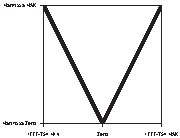
\includegraphics[width=0.7\textwidth]{Number line.pdf}
\end{center}

\ppara{As illustrated in FIG. \ref{fig:ieee_number_line}, the IEEE-754 sign-magnitude representation creates a fundamental discontinuity at zero. This visualization reveals how every value has an opposite representation—positive and negative—that differ only by the sign bit, creating a mirror of the entire number line. This includes cases like zero, which exists as both +0 and -0, despite attempting to represent the same mathematical value. This sign-magnitude approach introduces significant branching complexity in numerical operations, requiring separate code paths for different sign combinations and explicit testing of the sign for most arithmetic operations.}


\begin{lstlisting}[caption={Two's Complement Representation}, label={fig:spirix_number_line}]
\end{lstlisting}
\begin{center}
\begin{minipage}{0.49\textwidth}
  \centering
  \begin{adjustbox}{valign=t,width=\linewidth}
  \includegraphics[page=2]{Number line.pdf}
  \end{adjustbox}
\end{minipage}
\hfill
\begin{minipage}{0.49\textwidth}
  \centering
  \begin{adjustbox}{valign=t,width=\linewidth}
  \includegraphics[page=3]{Number line.pdf}
  \end{adjustbox}
\end{minipage}
\end{center}

\ppara{In contrast, FIG. \ref{fig:spirix_number_line}A presents a linear view of the invention's continuous two's complement representation. Unlike IEEE-754, the invention achieves a completely continuous number space where values wrap around to maintain mathematical relationships across the entire range, eliminating the discontinuity at zero. This continuity enables operations to cross the zero boundary without any special handling or branching.}

\ppara{FIG. \ref{fig:spirix_number_line}B further illustrates this concept with a vertically rotated perspective of the same representation, mapping values from fraction MAX/2+1 at the bottom to fraction MAX/2 at the top, with zero naturally landing in the middle. This visualization highlights how zero becomes a contiguous value in the number line rather than a special case requiring separate handling.}

\newpage
\subsection*{Core Configuration Definitions}

\ppara{The Scalar and Circle configurations form the core of the system. These definitions provide a unified framework for representing and operating on both real and complex numbers.}

\begin{lstlisting}[style=rust, caption={Scalar Type Definition}, label={fig:scalar_structure}]
pub struct Scalar<F: Integer, E: Integer> {
	/// The normalized fraction component representing the significand.
	/// The fraction size determines the precision of the value.
	/// The N (prefix bit) pattern determines the number's state
	/// (normal, exploded, vanished, Zero or undefined/unimplemented).
	pub fraction: F,

	/// The exponent component determining the scale of the value/phase.
	/// The exponent size determines the range of the value/phase.
	/// When equal to AMBIGUOUS_EXPONENT, indicates an escaped phase
	/// (exploded, vanished, undefined/unimplemented or Zero).
	pub exponent: E,
}
\end{lstlisting}

\ppara{As shown in FIG. \ref{fig:scalar_structure}, the Scalar type implements the representation for real numbers thru two primary components: a normalized two's complement fraction that determines precision, and an unbiased two's complement exponent that determines range. Unlike IEEE-754's sign-magnitude representation with a separate sign bit, the Scalar structure naturally encodes sign information within the fraction's two's complement representation. The parameterized design allows for independent selection of fraction and exponent sizes to match application requirements.}

\newpage
\begin{lstlisting}[style=rust, caption={Circle Type Definition}, label={fig:circle_structure}]
pub struct Circle<F: Integer, E: Integer> {
	/// The real phase representing the real part of the complex number.
	/// The normalization level of this component indicates current state
	/// (normal, exploded, vanished, undefined/unimplemented, Zero).
	pub real: F,

	/// The imaginary component representing the phase of i.
	/// The normalization level of this component indicates current state
	/// (normal, exploded, vanished, undefined/unimplemented, Zero).
	pub imaginary: F,

	/// The shared exponent component determining the scale of both phases.
	/// When equal to AMBIGUOUS_EXPONENT, indicates an escaped phase
	/// (exploded, vanished, undefined or Zero).
	pub exponent: E,
}
\end{lstlisting}

\ppara{FIG. \ref{fig:circle_structure} presents the Circle type implementation for complex numbers. The structure contains real and imaginary fractions sharing a common exponent, enabling efficient complex arithmetic operations while maintaining mathematical consistency. By using a shared exponent for both fractions, the Circle type maintains alignment between real and imaginary components, greatly simplifying complex arithmetic operations compared to traditional approaches that require separate handling for each component.}
\vfill
\begin{lstlisting}[style=rust, caption={Where fraction: F and exponent: E are any sized integer}, label={fig:integer}]
impl Integer for i8 {}
impl Integer for i16 {}
impl Integer for i32 {}
impl Integer for i64 {}
impl Integer for i128 {}
\end{lstlisting}

\ppara{The type flexibility of the invention is demonstrated in FIG. \ref{fig:integer}, showing how any integer size can be used for both fraction and exponent components. This abstraction over integer types allows the system to adapt to different precision and range requirements. While the implementation shown uses standard signed integer sizes (i8 thru i128), the system can work with arbitrary-sized integers, allowing for precise tuning of numeric representations to application-specific needs.}
\newpage
\begin{lstlisting}[caption={FE Type Configurations - Precision vs. Range}, label={fig:spirix_configurations}]
\end{lstlisting}
\begin{table}[ht]
\centering
\renewcommand{\arraystretch}{1.5}
\begin{tabular}{|c|c|c|c|c|c|}
\hline
\multirow{2}{*}{\textbf{Range}} & \multicolumn{5}{c|}{\textbf{Precision (Fraction Bits)}} \\
\cline{2-6}
 & \textbf{F3} & \textbf{F4} & \textbf{F5} & \textbf{F6} & \textbf{F7} \\
 & \small{2.2 digits} & \small{4.6 digits} & \small{9.4 digits} & \small{19 digits} & \small{38.3 digits} \\
\hline
\textbf{E3} & F3E3 & F4E3 & F5E3 & F6E3 & F7E3 \\
\small{$\approx 10^{\pm2.1}$} & \small{$\langle$i8, i8$\rangle$} & \small{$\langle$i16, i8$\rangle$} & \small{$\langle$i32, i8$\rangle$} & \small{$\langle$i64, i8$\rangle$} & \small{$\langle$i128, i8$\rangle$} \\
\hline
\textbf{E4} & F3E4 & F4E4 & F5E4 & F6E4 & F7E4 \\
\small{$\approx 10^{\pm4.5}$} & \small{$\langle$i8, i16$\rangle$} & \small{$\langle$i16, i16$\rangle$} & \small{$\langle$i32, i16$\rangle$} & \small{$\langle$i64, i16$\rangle$} & \small{$\langle$i128, i16$\rangle$} \\
\hline
\textbf{E5} & F3E5 & F4E5 & F5E5 & F6E5 & F7E5 \\
\small{$\approx 10^{\pm9.3}$} & \small{$\langle$i8, i32$\rangle$} & \small{$\langle$i16, i32$\rangle$} & \small{$\langle$i32, i32$\rangle$} & \small{$\langle$i64, i32$\rangle$} & \small{$\langle$i128, i32$\rangle$} \\
\hline
\textbf{E6} & F3E6 & F4E6 & F5E6 & F6E6 & F7E6 \\
\small{$\approx 10^{\pm18.9}$} & \small{$\langle$i8, i64$\rangle$} & \small{$\langle$i16, i64$\rangle$} & \small{$\langle$i32, i64$\rangle$} & \small{$\langle$i64, i64$\rangle$} & \small{$\langle$i128, i64$\rangle$} \\
\hline
\textbf{E7} & F3E7 & F4E7 & F5E7 & F6E7 & F7E7 \\
\small{$\approx 10^{\pm38.2}$} & \small{$\langle$i8, i128$\rangle$} & \small{$\langle$i16, i128$\rangle$} & \small{$\langle$i32, i128$\rangle$} & \small{$\langle$i64, i128$\rangle$} & \small{$\langle$i128, i128$\rangle$} \\
\hline
\end{tabular}
\end{table}

\ppara{FIG. \ref{fig:spirix_configurations} illustrates the precision-range matrix of valid FE type combinations. This table demonstrates how the invention enables independent configuration of precision (controlled by fraction size) and range (controlled by exponent size). From limited precision with wide range (F3E7) to high precision with narrower range (F7E3), the system accommodates diverse application requirements without forcing unnecessary compromises between precision and range.}

\ppara{Scalar values are calculated as:}
\ppara{$value = fraction \times 2^{exponent}$}

\ppara{Circle values have real and imaginary phases sharing a common exponent:}
\ppara{$value = (real + imaginary \times i) \times 2^{exponent}$}
\newpage
\subsection*{Normalization Levels and Numerical States}

\ppara{The invention employs a leading same bit normalization scheme to represent different numerical states thru specific bit patterns in the fraction component(s).}

\begin{lstlisting}[caption={Normalization Levels and Bit Patterns}, label={fig:normalization_levels}]
\end{lstlisting}
\begin{figure}[ht]
\centering
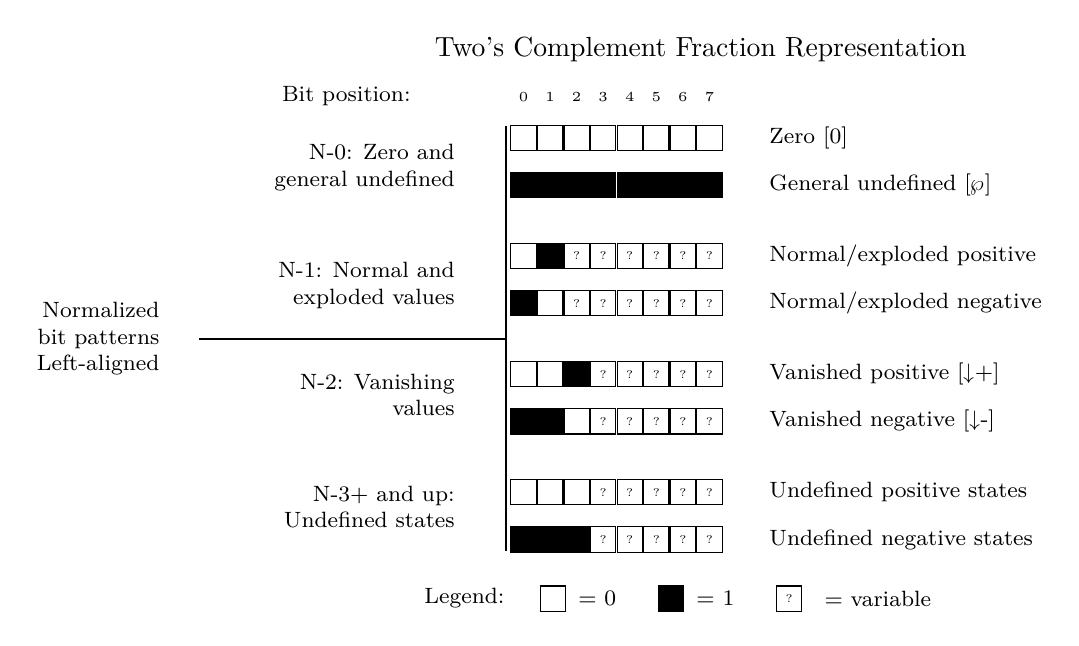
\begin{tikzpicture}[
    scale=0.75,
    every node/.style={font=\footnotesize},
    bit/.style={minimum width=0.4cm, minimum height=0.4cm, draw, anchor=center},
    highlight/.style={fill=black, text=white},
    empty/.style={fill=white},
    ]
    
    % Title
    \node at (4, 9.5) {\normalsize Two's Complement Fraction Representation};
    
    % Bit position markers
    \node[align=right] at (-2, 8.7) {Bit position:};
    \foreach \i in {0,...,7} {
        \node at (\i*0.45+1, 8.7) {\tiny \i};
    }
    
    % N-0: Zero and general undefined
    \node[align=right, anchor=east] at (0, 7.5) {N-0: Zero and\\general undefined};
    
    % Zero pattern
    \foreach \i in {0,...,7} {
        \node[bit, empty, scale=0.8] at (\i*0.45+1, 8) {};
    }
    \node[align=left, anchor=west] at (5, 8) {Zero [0]};
    
    % Undefined pattern
    \foreach \i in {0,...,7} {
        \node[bit, highlight, scale=0.8] at (\i*0.45+1, 7.2) {};
    }
    \node[align=left, anchor=west] at (5, 7.2) {General undefined [$\wp$]};
    
    % N-1: Normal and exploded values
    \node[align=right, anchor=east] at (0, 5.5) {N-1: Normal and\\exploded values};
    
    % Positive normal/exploded pattern
    \node[bit, empty, scale=0.8] at (1, 6) {};
    \node[bit, highlight, scale=0.8] at (1.45, 6) {};
    \foreach \i in {2,...,7} {
        \node[bit, scale=0.8] at (\i*0.45+1, 6) {\tiny?};
    }
    \node[align=left, anchor=west] at (5, 6) {Normal/exploded positive};
    
    % Negative normal/exploded pattern
    \node[bit, highlight, scale=0.8] at (1, 5.2) {};
    \node[bit, empty, scale=0.8] at (1.45, 5.2) {};
    \foreach \i in {2,...,7} {
        \node[bit, scale=0.8] at (\i*0.45+1, 5.2) {\tiny?};
    }
    \node[align=left, anchor=west] at (5, 5.2) {Normal/exploded negative};
    
    % N-2: Vanishing values
    \node[align=right, anchor=east] at (0, 3.65) {N-2: Vanishing\\values};
    
    % Positive vanished pattern
    \node[bit, empty, scale=0.8] at (1, 4) {};
    \node[bit, empty, scale=0.8] at (1.45, 4) {};
    \node[bit, highlight, scale=0.8] at (1.9, 4) {};
    \foreach \i in {3,...,7} {
        \node[bit, scale=0.8] at (\i*0.45+1, 4) {\tiny?};
    }
    \node[align=left, anchor=west] at (5, 4) {Vanished positive [$\downarrow$+]};
    
    % Negative vanished pattern
    \node[bit, highlight, scale=0.8] at (1, 3.2) {};
    \node[bit, highlight, scale=0.8] at (1.45, 3.2) {};
    \node[bit, empty, scale=0.8] at (1.9, 3.2) {};
    \foreach \i in {3,...,7} {
        \node[bit, scale=0.8] at (\i*0.45+1, 3.2) {\tiny?};
    }
    \node[align=left, anchor=west] at (5, 3.2) {Vanished negative [$\downarrow$-]};
    
    % N-3+: Specific undefined states
    \node[align=right, anchor=east] at (0, 1.75) {N-3+ and up:\\Undefined states};
    
    % Positive undefined patterns
    \node[bit, empty, scale=0.8] at (1, 2) {};
    \node[bit, empty, scale=0.8] at (1.45, 2) {};
    \node[bit, empty, scale=0.8] at (1.9, 2) {};
    \foreach \i in {3,...,7} {
        \node[bit, scale=0.8] at (\i*0.45+1, 2) {\tiny?};
    }
    \node[align=left, anchor=west] at (5, 2) {Undefined positive states};
    
    % Negative undefined patterns
    \node[bit, highlight, scale=0.8] at (1, 1.2) {};
    \node[bit, highlight, scale=0.8] at (1.45, 1.2) {};
    \node[bit, highlight, scale=0.8] at (1.9, 1.2) {};
    \foreach \i in {3,...,7} {
        \node[bit, scale=0.8] at (\i*0.45+1, 1.2) {\tiny?};
    }
    \node[align=left, anchor=west] at (5, 1.2) {Undefined negative states};
    
    \draw [thick] (0.7,8.2) -- (0.7,1);
    \draw [thick] (0.7,4.6) -- (-4.5,4.6);
    \node [align=right, anchor=east] at (-5, 4.6) {Normalized\\bit patterns\\Left-aligned};
    
    % Legend
    \node at (0, 0.2) {Legend:};
    \node[bit, empty, scale=0.8] at (1.5, 0.2) {};
    \node at (2.25, 0.2) {= 0};
    \node[bit, highlight, scale=0.8] at (3.5, 0.2) {};
    \node at (4.25, 0.2) {= 1};
    \node[bit, scale=0.8] at (5.5, 0.2) {\tiny?};
    \node at (7, 0.2) {= variable};
    
\end{tikzpicture}
\end{figure}
\vfill
\ppara{As depicted in FIG. \ref{fig:normalization_levels}, the normalization levels (N-levels) encode different numerical states thru distinct bit patterns in the most significant positions of the fraction. Normal values use N-1 normalization with bit patterns 01... or 10... in the most significant positions, while vanished values use N-2 normalization, and various undefined states are represented thru higher normalization levels. This normalization scheme allows for efficient state detection thru examination of the leading bits, eliminating the need for extensive branching logic and special case handling that characterizes IEEE-754 implementations.}

\ppara{A key innovation in the normalization scheme is the concept of "escaped" values—those that exceed normal representation range, but their phase is known. Unlike IEEE-754, which uses special values like infinity or NaN that lose information about the operation, the invention's escaped values preserve phase/orientation information, enabling continued participation in absolute operations with magnitudes outside normal range. For example a negative vanished Scalar multiplied by another negative vanished Scalar will never return zero ([$\downarrow$] $\cdot$ [$\downarrow$] != [0]) and the result will be a positive vanished Scalar ([-$\downarrow$] $\cdot$ [-$\downarrow$] $\rightarrow$ [+$\downarrow$]), thus preserving orientation and continuity from zero to infinity wherever possible.}

\newpage
\subsection*{Unified Treatment of Zero [0] and Infinity [$\infty$]}

\ppara{The invention implements a mathematically consistent approach to the singularities of zero and infinity. Unlike IEEE-754, which treats these values as special cases with separate positive and negative variants, the invention incorporates zero and infinity within its continuous mathematical framework.}

\ppara{Zero is represented as a specific bit pattern with all zeroes in the fraction, paired with an AMBIGUOUS\_EXPONENT. This approach treats zero as a singular point on the continuous number line rather than as two distinct values (+0 and -0) that require special handling. This unification eliminates the inconsistencies that arise in IEEE-754 when operations involving positive and negative zeros produce different results.}

\ppara{Similarly, infinity is represented as a specific bit pattern within the fraction component, also with an AMBIGUOUS\_EXPONENT. The system maintains consistent mathematical relationships involving infinity, such as:}

\ppara{- Any non-zero value divided by zero produces infinity}
\ppara{- Infinity multiplied by any non-zero value remains infinity}
\ppara{- Zero divided by any non-zero value remains zero}
\ppara{- Adding or subtracting infinity with anything produces an undefined result with a specific bit pattern preserving the cause}

\ppara{By treating both zero and infinity as orientationless singular points, the invention enables consistent behavior across all operations, greatly reducing the special case handling while preserving mathematical coherence beyond the boundaries of representable values.}

\newpage
\subsection*{Undefined States and Error Preservation}

\begin{lstlisting}[style=rust, caption={Excerpt of Undefined State Definitions}, label={fig:undefined}]
// L3 Basic operators
/// ¡$\square\square\square\blacksquare\blacksquare\blacksquare\blacksquare\blacksquare$¡
pub const EXPLODED_PLUS_EXPLODED: Undefined = Undefined {
	prefix: 0b00011111u8 as i8,
	symbol: "¡$\wp$¡ ¡$\uparrow$¡+¡$\uparrow$¡",
	description: "Exploded value addition with exploded value",
};
/// ¡$\blacksquare\blacksquare\blacksquare\square\square\square\square\square$¡
pub const EXPLODED_MINUS_EXPLODED: Undefined = Undefined {
	prefix: 0b11100000u8 as i8,
	symbol: "¡$\wp$¡ ¡$\uparrow$¡-¡$\uparrow$¡",
	description: "Exploded value subtraction with exploded value",
};
/// ¡$\square\square\square\blacksquare\blacksquare\blacksquare\blacksquare\square$¡
pub const VANISHED_PLUS_VANISHED: Undefined = Undefined {
	prefix: 0b00011110u8 as i8,
	symbol: "¡$\wp$¡ ¡$\downarrow$¡+¡$\downarrow$¡",
	description: "Vanished value addition with vanished value",
};
/// ¡$\blacksquare\blacksquare\blacksquare\square\square\square\square\blacksquare$¡
pub const VANISHED_MINUS_VANISHED: Undefined = Undefined {
	prefix: 0b11100001u8 as i8,
	symbol: "¡$\wp$¡ ¡$\downarrow$¡-¡$\downarrow$¡",
	description: "Vanished value subtraction with vanished value",
};
// L4 Powers and roots
/// ¡$\square\square\square\square\blacksquare\blacksquare\blacksquare\blacksquare$¡
pub const EXPLODED_POWER: Undefined = Undefined {
	prefix: 0b00001111u8 as i8,
	symbol: "¡$\wp$¡ ¡$\uparrow$¡^",
	description: "Exploded value raised to power",
};
/// ¡$\blacksquare\blacksquare\blacksquare\blacksquare\square\square\square\square$¡
pub const VANISHED_POWER: Undefined = Undefined {
	prefix: 0b11110000u8 as i8,
	symbol: "¡$\wp$¡ ¡$\downarrow$¡^",
	description: "Vanished value raised to power",
};
/// ¡$\square\square\square\square\blacksquare\blacksquare\blacksquare\square$¡
pub const POWER_EXPLODED: Undefined = Undefined {
	prefix: 0b00001110u8 as i8,
	symbol: "¡$\wp$¡ ^¡$\uparrow$¡",
	description: "Value raised to exploded power",
};
// L5 Logarithms
/// ¡$\square\square\square\square\square\blacksquare\blacksquare\blacksquare$¡
pub const EXPLODED_LOG: Undefined = Undefined {
	prefix: 0b00000111u8 as i8,
	symbol: "¡$\wp$¡ ¡$\uparrow$¡@",
	description: "Logarithm of exploded value",
};
/// ¡$\blacksquare\blacksquare\blacksquare\blacksquare\blacksquare\square\square\square$¡
pub const VANISHED_LOG: Undefined = Undefined {
	prefix: 0b11111000u8 as i8,
	symbol: "¡$\wp$¡ ¡$\downarrow$¡@",
	description: "Logarithm of vanished value",
};
/// ¡$\square\square\square\square\square\blacksquare\blacksquare\square$¡
pub const LOG_EXPLODED: Undefined = Undefined {
	prefix: 0b00000110u8 as i8,
	symbol: "¡$\wp$¡ @¡$\uparrow$¡",
	description: "Logarithm with exploded base",
};
// L6 Sine/Cosine
/// ¡$\square\square\square\square\square\square\blacksquare\blacksquare$¡
pub const SINE: Undefined = Undefined {
	prefix: 0b00000011u8 as i8,
	symbol: "¡$\wp$¡ s",
	description: "Sine of value with imprecise period position",
};
/// ¡$\blacksquare\blacksquare\blacksquare\blacksquare\blacksquare\blacksquare\square\square$¡
pub const COSINE: Undefined = Undefined {
	prefix: 0b11111100u8 as i8,
	symbol: "¡$\wp$¡ c",
	description: "Cosine of value with imprecise period position",
};
\end{lstlisting}

\ppara{One of the most significant innovations of the invention is its approach to undefined numerical states, as illustrated in FIG. \ref{fig:undefined}. Unlike IEEE-754's single NaN (Not a Number) representation, which collapses all error conditions into a single state, the system employs distinct bit patterns to encode the specific cause of undefined operations. The figure demonstrates how different operations that produce undefined results (such as 0/0, $\infty$-$\infty$, or 0\^{}0) are assigned unique bit patterns in the fraction component, always paired with the AMBIGUOUS\_EXPONENT.}

\ppara{This preservation of error cause enables error tracing in numerical applications. When an undefined result propagates thru subsequent operations, the system maintains the original cause rather than losing this critical information, allowing developers to trace computational issues to their source. The hierarchical organization of undefined states further enhances this capability, with different operations (basic arithmetic, powers, logarithms, trigonometric functions) assigned different ranges within the bit pattern space. Each of these patterns, given sufficient fraction size can provide other important undefined information or custom implemented behavior.}
\newpage
\subsection*{SPIRIX Operation Truth Tables}

\ppara{The invention attempts to implement consistent and helpful behavior across numerical operations and states. The SPIRIX Circle and Scalar states follow Riemann principles when performing operations.}

\vfill
\begin{lstlisting}[caption={SPIRIX Addition Operation Truth Table}, label={fig:addition_table}]
\end{lstlisting}
\begin{center}
    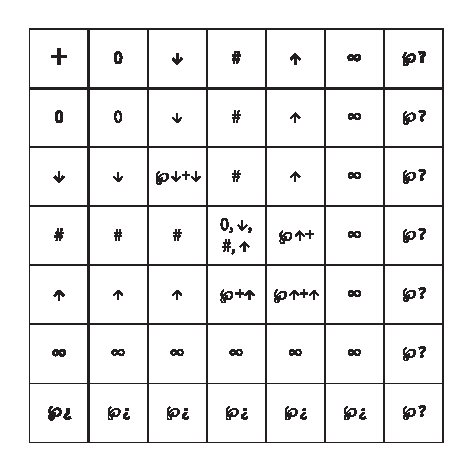
\includegraphics[width=0.8\textwidth]{addition truth table.pdf}
\end{center}
\ppara{FIG. \ref{fig:addition_table} above presents the Addition Operation Truth Table, illustrating how different states interact under addition in the SPIRIX system. The table demonstrates the mathematical consistency of addition across normal, vanished, exploded, and special states. Note that operations between certain states, such as adding an exploded and a normal, produce specific undefined states, preserving information about the operation that led to the undefined state.}

\newpage
\begin{lstlisting}[caption={SPIRIX Subtraction Operation Truth Table}, label={fig:subtraction_table}]
\end{lstlisting}
\begin{center}
    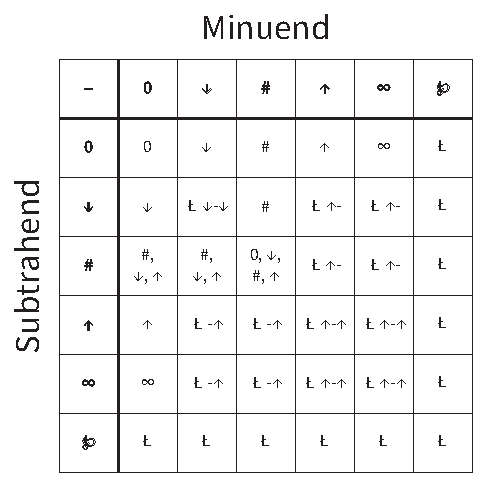
\includegraphics[width=0.8\textwidth]{subtraction truth table.pdf}
\end{center}
\ppara{The Subtraction Operation Truth Table in FIG. \ref{fig:subtraction_table} shows the outcomes of subtracting different states in the SPIRIX system. The minuend (value being subtracted from) appears along the top, and the subtrahend (value being subtracted) appears along the left column. The table highlights how subtraction maintains mathematical coherence even in boundary cases, Note the minimum negative and minimum positive explode or vanish upon negation of the subtrahend.}

\newpage
\begin{lstlisting}[caption={SPIRIX Multiplication Operation Truth Table}, label={fig:multiplication_table}]
\end{lstlisting}
\begin{center}
    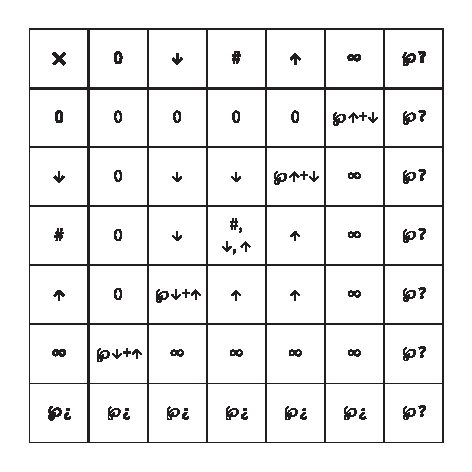
\includegraphics[width=0.8\textwidth]{multiplication truth table.pdf}
\end{center}
\ppara{FIG. \ref{fig:multiplication_table} demonstrates the system's multiplicative consistency thru the Multiplication Operation Truth Table. A key feature illustrated in this table is that the product of two non-zero states is never a zero state, preserving a fundamental mathematical property that can be violated in IEEE-754 implementations due to multiplicative underflow to zero or overflow to infinity. The table also shows how the system maintains phase information even when results exceed normal range, transitioning to exploded or vanished states rather than truncating to infinity or zero.}

\newpage
\begin{lstlisting}[caption={SPIRIX Division Operation Truth Table}, label={fig:division_table}]
\end{lstlisting}
\begin{center}
    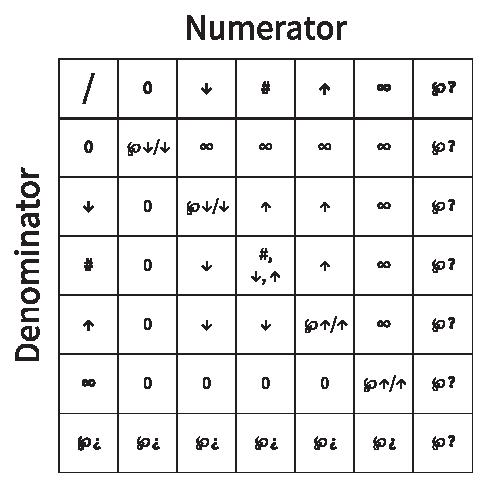
\includegraphics[width=0.8\textwidth]{division truth table.pdf}
\end{center}
\ppara{The Division Operation Truth Table in FIG. \ref{fig:division_table} illustrates division behavior for all Circle and Scalar states. The table shows how division by zero produces infinity for non-zero numerators, while division of zero by any non-zero value produces zero. Division operations between escaped values (exploded and vanished) follow Riemann principles, with vanished divided by exploded producing vanished, and exploded divided by vanished producing exploded. This behavior eliminates many special cases that would otherwise require explicit handling in many numerical applications.}
\newpage
\begin{lstlisting}[caption={SPIRIX Number Line and Comparison Order}, label={fig:spirix_ordering}]
\end{lstlisting}
\begin{figure}[htbp]
  \centering
  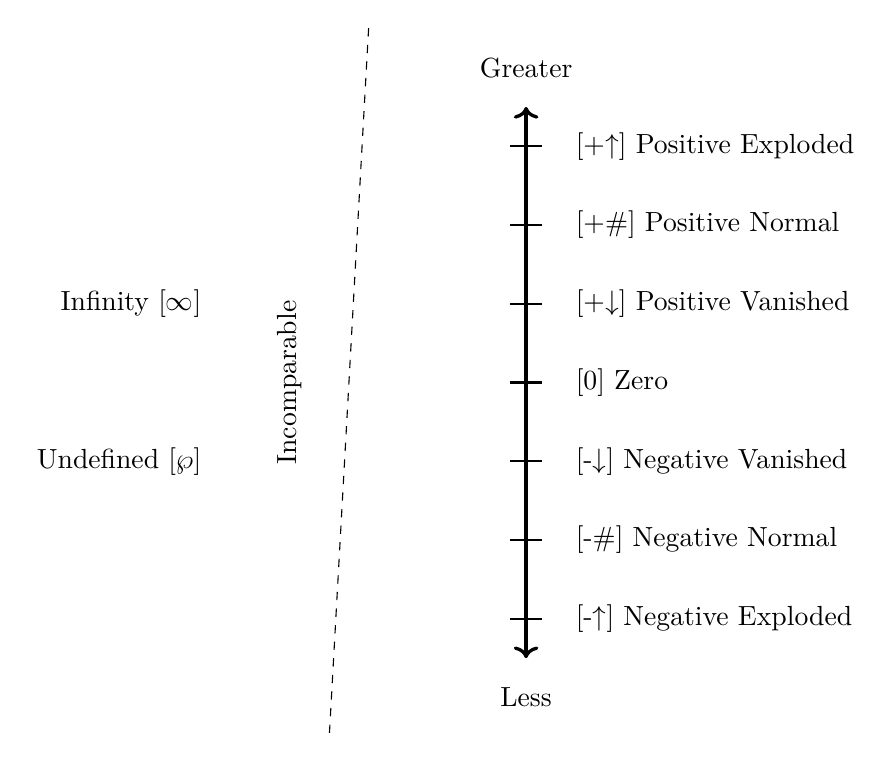
\begin{tikzpicture}[scale=1]

    \draw[<->, very thick] (0,-3.5) -- (0,3.5);
    \node[centered] at (0,4) {Greater};
    \node[centered] at (0,-4) {Less};
    
    \draw[thick] (-0.2,3) -- (0.2,3) node[right=0.3cm] {[+$\uparrow$] Positive Exploded};
    \draw[thick] (-0.2,2) -- (0.2,2) node[right=0.3cm] {[+\#] Positive Normal};
    \draw[thick] (-0.2,1) -- (0.2,1) node[right=0.3cm] {[+$\downarrow$] Positive Vanished};
    \draw[thick] (-0.2,0) -- (0.2,0) node[right=0.3cm] {[0] Zero};
    \draw[thick] (-0.2,-1) -- (0.2,-1) node[right=0.3cm] {[-$\downarrow$] Negative Vanished};
    \draw[thick] (-0.2,-2) -- (0.2,-2) node[right=0.3cm] {[-\#] Negative Normal};
    \draw[thick] (-0.2,-3) -- (0.2,-3) node[right=0.3cm] {[-$\uparrow$] Negative Exploded};
    \node[left] at (-4,1) {Infinity [$\infty$]};
    \node[left] at (-4,-1) {Undefined [$\wp$]};

    \draw[dashed] (-2,4.5) -- (-2.5,-4.5);
    \node[rotate=90] at (-3,0) {Incomparable};

    
  \end{tikzpicture}
\end{figure}
\ppara{FIG. \ref{fig:spirix_ordering} presents the SPIRIX Scalar number line and comparison ordering, illustrating the continuous nature of the two's complement representation. This figure illustrates how normal, vanished, and exploded values maintain a consistent ordering relationship with a singular zero, while infinity and undefined states remain incomparable.}
\vfill
\subsection*{IEEE-754 vs. SPIRIX Implementation Complexity}

\ppara{The fundamental differences in representation approach between IEEE-754 and the invention result in significant implementation differences, particularly in terms of control flow complexity and instruction count.}

\newpage
\begin{lstlisting}[caption={IEEE-754 Binary32 Subtraction Flowchart}, label={fig:ieee_subtract_flowchart}]
\end{lstlisting}
\begin{figure}[htbp]
  \centering
  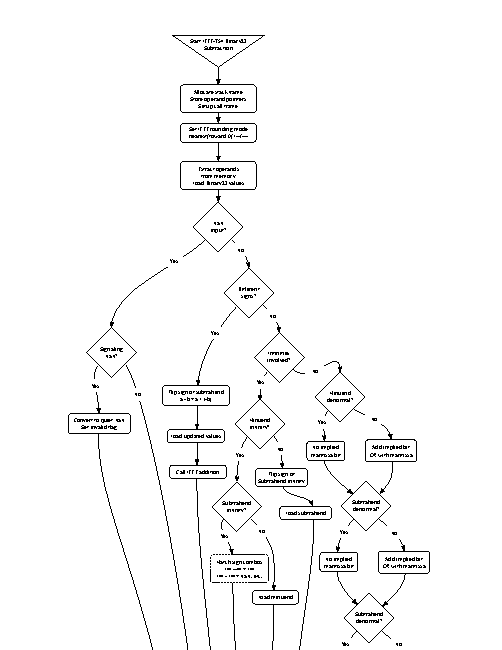
\includepdf[pages=1, scale=0.85]{IEEE subtract flowchart.pdf}
\end{figure}
\newpage
\begin{figure}[htbp]
  \centering
  \includepdf[pages=2, scale=0.85]{IEEE subtract flowchart.pdf}
\end{figure}
\newpage
\begin{figure}[htbp]
  \centering
  \includepdf[pages=3, scale=0.85]{IEEE subtract flowchart.pdf}
\end{figure}
\newpage

\ppara{FIG. \ref{fig:ieee_subtract_flowchart} illustrates the elaborate control flow required for IEEE-754 subtraction operations. The flowchart reveals numerous branching paths needed to handle different sign combinations, exponent comparisons, and special value cases. This complexity stems directly from IEEE-754's sign-magnitude representation, which creates distinct processing paths for different sign combinations and requires explicit sign bit testing for virtually all operations.}
\vfill
\ppara{In contrast, FIG. \ref{fig:scalar_subtract_flowchart} demonstrates the control flow of Scalar subtraction. The diagram shows two primary paths: one for normal values and one for ambiguous cases, with the normal path aligning and subtracting fractions, then checking and updating the exponent without denormal, sign, exponent bias or implied one steps. Note how addition and subtraction only need to check for underflow. Overflow is naturally handled by the placement of the AMBIGUOUS\_EXPONENT where the largest magnitude wraps around to our ambiguous value.}
\newpage
\begin{lstlisting}[caption={Scalar Subtraction Flowchart}, label={fig:scalar_subtract_flowchart}]
\end{lstlisting}
\begin{figure}[htbp]
  \centering
  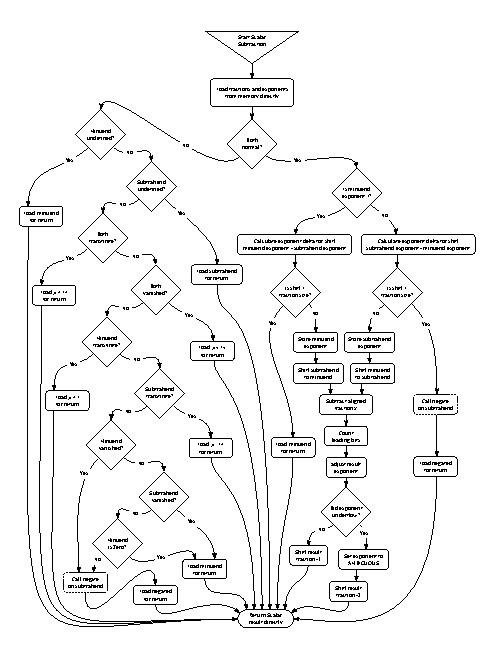
\includepdf[pages=1, scale=0.85]{Scalar subtract flowchart.pdf}
\end{figure}
\newpage

\begin{lstlisting}[style=rust, caption={Annotated IEE-754 Binary32 Normal Subtraction ASM Trace}, label={fig:ieee_subtract}]
; Main Subtraction Fuction Entry Point
[001]sub rsp, 0x58                 ; Allocate 88 bytes on the stack
[002]mov qword ptr [rsp 0x8], rdi  ; Store first parameter (pointer to first value)
[003]mov al, dl                    ; Move the 3rd parameter (lower byte) to al
[004]mov dword ptr [rsp 0x18], esi ; Store second parameter (second value)
[005]mov ecx, dword ptr [rsp 0x18] ; Load second Binary32 value into ecx
[006]mov dword ptr [rsp 0x14], ecx ; Store second Binary32 value at rsp+20
[007]mov byte ptr [rsp 0x1f], al   ; Store lower byte of 3rd parameter at rsp+31
[008]mov qword ptr [rsp 0x30], rdi ; Move first parameter
[009]lea rax, ptr [rip 0x3d6e9]    ; Load effective address
[010]lea rdi, ptr [rsp 0x1f]       ; Load address of next function into rdi
[011]call rax                      ; Call function at address in rax

; Set Rounding Mode
[012]push rax                 ; Save rax register
[013]mov qword ptr [rsp], rdi ; Store rdi at top of stack
[014]call 0x558bdf671e20      ; Call function to set rounding mode

; Convert Rounding Mode to Float Format
[015]mov qword ptr [rsp-0x8], rdi      ; Store rdi at rsp-8
[016]movzx eax, byte ptr [rdi]         ; Zero-extend byte at [rdi] into eax
[017]mov qword ptr [rsp-0x18], rax     ; Store extended value at rsp-24
[018]mov rax, qword ptr [rsp-0x18]     ; Load value from rsp-24 into rax
[019]lea rcx, ptr [rip 0x452af]        ; Load effective address (jump table?)
[020]movsxd rax, dword ptr [rcx rax*4] ; Load and sign-extend value from jump table
[021]add rax, rcx                      ; Add base address to jump offset
[022]jmp rax                           ; Jump to the calculated address
[023]mov byte ptr [rsp-0x9], 0x0       ; Set byte at rsp-9 to 0
[024]jmp 0x558bdf671e65                ; Jump to function epilogue
[025]mov al, byte ptr [rsp-0x9]        ; Load byte from rsp-9 into al
[026]ret                               ; Return from function

; Set Rounding Mode
[027]movzx edi, al                ; Zero-extend al into edi
[028]call qword ptr [rip 0x5bf45] ; Call function pointer at rip+0x5bf45

; Rounding Mode Helper
[029]push rbp                     ; Save base pointer
[030]mov rbp, rsp                 ; Set new base pointer
[031]push rbx                     ; Save rbx register
[032]sub rsp, 0x8                 ; Allocate 8 bytes on stack
[033]mov ebx, edi                 ; Store first parameter in ebx
[034]mov rax, qword ptr fs:[0x0]  ; Load value from fs segment
[035]lea rax, ptr [rax-0x4f]      ; Calculate address at fs:0 - 79
[036]mov byte ptr [rax], bl       ; Store lowest byte of ebx at calculated address
[037]mov rbx, qword ptr [rbp-0x8] ; Restore rbx
[038]leave                        ; Restore stack and base pointer
[039]ret                          ; Return from function

; Set Rounding Mode (continued)
[040]pop rax ; Restore rax
[041]ret     ; Return from function

; Main Subtraction Function (continued)
[042]jmp 0x558bdf63473a            ; Jump to next part of subtraction function
[043]mov rax, qword ptr [rsp 0x8]  ; Load pointer to first Binary32 from rsp+8
[044]mov eax, dword ptr [rax]      ; Load value of first Binary32 into eax
[045]mov dword ptr [rsp 0x28], eax ; Store first Binary32 at rsp+40
[046]lea rdi, ptr [rsp 0x14]       ; Load address of second value into rdi
[047]call 0x558bdf6346e0           ; Call function to borrow memory value

; Borrow Memory Value
[048]mov rax, rdi                 ; Copy input parameter to rax
[049]mov qword ptr [rsp-0x8], rax ; Store rax at rsp-8
[050]ret                          ; Return from function

; Main Subtraction Function (continued)
[051]mov qword ptr [rsp], rax      ; Store return value at top of stack
[052]jmp 0x558bdf634755            ; Jump to next part of subtraction
[053]mov rax, qword ptr [rsp]      ; Load pointer from stack into rax
[054]mov eax, dword ptr [rax]      ; Load value at pointer into eax
[055]mov dword ptr [rsp 0x2c], eax ; Store second Binary32 at rsp+44
[056]mov eax, dword ptr [rsp 0x28] ; Load first Binary32 into eax
[057]mov dword ptr [rsp 0x4c], eax ; Store first Binary32 at rsp+76
[058]mov edi, dword ptr [rsp 0x4c] ; Load first value into edi
[059]mov eax, dword ptr [rsp 0x2c] ; Load second Binary32 into eax
[060]mov dword ptr [rsp 0x50], eax ; Store second Binary32 at rsp+80
[061]mov esi, dword ptr [rsp 0x50] ; Load second value into esi
[062]call qword ptr [rip 0x9906b]  ; Call function for low-level

; Low-level Float Subtraction
[063]push rbp            ; Save base pointer
[064]mov rbp, rsp        ; Set new base pointer
[065]mov eax, edi        ; Copy first Binary32 to eax
[066]mov edx, esi        ; Copy second Binary32 to edx
[067]xor esi, edi        ; XOR the two Binary32 values
[068]js 0x558bdf671e83   ; Jump if sign bit is set (opposing signs)
[069]mov rsi, rdx        ; Copy second Binary32 to rsi
[070]mov rdi, rax        ; Copy first Binary32 to rdi
[071]call 0x558bdf6721a9 ; Call function to add float magnitudes

; Add Float Magnitudes
[072]push rbp            ; Save base pointer
[073]mov rbp, rsp        ; Set new base pointer
[074]mov rcx, rdi        ; Copy first Binary32 to rcx
[075]shr rcx, 0x17       ; Shift right by 23 bits (extract exponent)
[076]movzx ecx, cl       ; Zero-extend lowest byte to get 8-bit exponent
[077]mov r9, rcx         ; Copy exponent to r9
[078]mov r10, rdi        ; Copy first Binary32 to r10
[079]and r10d, 0x7fffff  ; Mask to get mantissa (23 bits)
[080]mov rax, rsi        ; Copy second Binary32 to rax
[081]shr rax, 0x17       ; Shift right by 23 bits (extract exponent)
[082]movzx eax, al       ; Zero-extend lowest byte to get 8-bit exponent
[083]mov rdx, rsi        ; Copy second Binary32 to rdx
[084]and edx, 0x7fffff   ; Mask to get mantissa (23 bits)
[085]mov r11, rcx        ; Copy first exponent to r11
[086]sub r11, rax        ; Subtract exponents (for comparing magnitude)
[087]jnz 0x558bdf67224f  ; Jump if exponents are different
[088]mov r8d, edi        ; Copy first Binary32 to r8d
[089]shr r8d, 0x1f       ; Shift right by 31 bits (extract sign bit)
[090]shl r10, 0x6        ; Shift first mantissa left by 6 bits (normalize)
[091]shl rdx, 0x6        ; Shift second mantissa left by 6 bits (normalize)
[092]test r11, r11       ; Test if exponent difference is Zero
[093]js 0x558bdf6722c4   ; Jump if exponent difference is negative
[094]cmp rax, 0xff       ; Check for NaN/Infinity
[095]jz 0x558bdf67230b   ; Jump if second number is NaN or Infinity
[096]test rcx, rcx       ; Test if first exponent is Zero
[097]mov esi, 0x20000000 ; Set esi to 0x20000000 (implied 1 for normal numbers)
[098]cmovz rsi, r10      ; True for normals, false for subnormal
[099]mov rdi, rax        ; Copy second exponent to rdi
[100]sub rdi, rcx        ; Calculate exponent difference
[101]add rsi, r10        ; Add implied 1 to first mantissa
[102]cmp rdi, 0x1e       ; Compare exponent difference with 30
[103]jnbe 0x558bdf672327 ; Jump if difference is not within range
[104]mov ecx, edi        ; Copy exponent difference to ecx
[105]neg ecx             ; Negate exponent difference
[106]mov r9d, esi        ; Copy first mantissa with implied 1 to r9d
[107]shl r9d, cl         ; Shift left by exponent difference
[108]test r9d, r9d       ; Test if shifted value is Zero
[109]setnz r10b          ; Set r10b to 1 if not Zero, 0 if Zero
[110]movzx r10d, r10b    ; Zero-extend r10b to r10d
[111]mov ecx, edi        ; Copy exponent difference to ecx
[112]shr esi, cl         ; Shift first mantissa right by exponent difference
[113]or r10d, esi        ; Combine shifted bits with sticky bit
[114]mov r10d, r10d      ; Clear upper 32 bits of r10
[115]mov r9, rax         ; Copy second exponent to r9
[116]jmp 0x558bdf6722a3  ; Jump to next part of float addition
[117]lea rdx, ptr [r10 rdx*1 0x20000000] ; Calculate sum of mantissas
[118]cmp rdx, 0x3fffffff ; Check if result needs normalization
[119]jnbe 0x558bdf67220e ; Jump if normalization needed
[120]movzx edi, r8b      ; Zero-extend sign bit to edi
[121]mov rsi, r9         ; Copy exponent to rsi
[122]call 0x558bdf671f65 ; Call function to round and pack to Binary32 format

; Round and Pack to Binary32 Format
[123]push rbp                      ; Save base pointer
[124]mov rbp, rsp                  ; Set new base pointer
[125]push r15                      ; Save r15 register
[126]push r14                      ; Save r14 register
[127]push r13                      ; Save r13 register
[128]push r12                      ; Save r12 register
[129]push rbx                      ; Save rbx register
[130]sub rsp, 0x18                 ; Allocate 24 bytes on stack
[131]mov r15d, edi                 ; Store sign bit in r15d
[132]mov dword ptr [rbp-0x34], edi ; Store sign bit at rbp-52
[133]mov rbx, rsi                  ; Store exponent in rbx
[134]mov r13, rdx                  ; Store mantissa in r13
[135]mov rax, qword ptr fs:[0x0]   ; Load value from fs segment
[136]lea rax, ptr [rax-0x4f]       ; Calculate address at fs:0 - 79
[137]movzx r14d, byte ptr [rax]    ; Load rounding mode into r14d
[138]test r14b, r14b               ; Test if rounding mode is 0 (to nearest)
[139]setz byte ptr [rbp-0x40]      ; Set flag at rbp-64 if rounding mode is 0
[140]mov r12d, 0x40                ; Set r12d to 64 (used for rounding)
[141]test r14b, 0xfb               ; Test rounding mode against 0xfb
[142]jz 0x558bdf671fc9             ; Jump if specific rounding mode
[143]mov r15d, r13d                ; Copy mantissa to r15d
[144]and r15d, 0x7f                ; Mask with 0x7f (7 least significant bits)
[145]mov dword ptr [rbp-0x38], ebx ; Store exponent at rbp-56
[146]cmp ebx, 0xfc                 ; Compare exponent with 0xfc
[147]jbe 0x558bdf672000            ; Jump if exponent <= 0xfc
[148]movzx r12d, r12b              ; Zero-extend r12b to r12d
[149]add r12, r13                  ; Add mantissa to r12
[150]shr r12, 0x7                  ; Shift right by 7 bits (rounding)
[151]test r15b, r15b               ; Test if lower 7 bits are Zero
[152]jnz 0x558bdf6720ec            ; Jump if lower 7 bits are not Zero
[153]mov rax, qword ptr fs:[0x0]   ; Load value from fs segment
[154]lea rax, ptr [rax-0x50]       ; Calculate address at fs:0 - 80
[155]or byte ptr [rax], 0x1        ; Set inexact flag
[156]cmp r14b, 0x6                 ; Compare rounding mode with 6
[157]jnz 0x558bdf672014            ; Jump if rounding mode is not 6
[158]cmp r15b, 0x40                ; Compare lower 7 bits with 0x40
[159]setz al                       ; Set al to 1 if equal, 0 if not
[160]movzx eax, al                 ; Zero-extend al to eax
[161]and rax, qword ptr [rbp-0x40] ; AND with rounding flag
[162]not rax                       ; Complement result
[163]and r12, rax                  ; Mask r12 with result
[164]mov eax, 0x0                  ; Set eax to 0
[165]cmovz rbx, rax                ; If Zero, set exponent to 0
[166]mov eax, dword ptr [rbp-0x34] ; Load sign bit into eax
[167]shl eax, 0x1f                 ; Shift sign bit to position 31
[168]shl ebx, 0x17                 ; Shift exponent to position 23-30
[169]add eax, ebx                  ; Combine sign and exponent
[170]mov eax, eax                  ; Clear upper 32 bits
[171]add rax, r12                  ; Add mantissa to result
[172]add rsp, 0x18                 ; Deallocate stack space
[173]pop rbx                       ; Restore rbx
[174]pop r12                       ; Restore r12
[175]pop r13                       ; Restore r13
[176]pop r14                       ; Restore r14
[177]pop r15                       ; Restore r15
[178]pop rbp                       ; Restore base pointer
[179]ret                           ; Return from function

; Add Float Magnitudes (epilogue)
[180]pop rbp ; Restore base pointer
[181]ret     ; Return from function

; Low-level Float Subtraction (epilogue)
[182]jmp 0x558bdf671e81 ; Jump to another part of function
[183]pop rbp            ; Restore base pointer
[184]ret                ; Return from function

; Main Subtraction Function (epilogue)
[185]mov dword ptr [rsp 0x54], eax ; Store result at rsp+84
[186]mov eax, dword ptr [rsp 0x54] ; Load result back into eax
[187]mov dword ptr [rsp 0x24], eax ; Store result at rsp+36
[188]mov eax, dword ptr [rsp 0x24] ; Load result back into eax
[189]mov dword ptr [rsp 0x20], eax ; Store result at rsp+32
[190]mov eax, dword ptr [rsp 0x20] ; Load result back into eax
[191]add rsp, 0x58                 ; Deallocate 88 bytes from stack
[192]ret                           ; Return from function

\end{lstlisting}

\ppara{The assembly instruction trace above for IEEE-754 Binary32 subtraction in FIG. \ref{fig:ieee_subtract} further highlights the implementation complexity of IEEE-754 floating-point operations. The trace reveals approximately 192 machine instructions with complicated branching even for this normal case. This trace has 7 function calls, 6 unconditional jumps, 10 conditional jumps, and 7 returns, creating potential pipeline stalls and prediction failures in modern processors.}
\vfill
\ppara{FIG. \ref{fig:scalar_subtract} below presents the assembly implementation of Scalar subtraction using the invention's two's complement method. The assembly instructions demonstrate how most normal cases can be completed in 33 instructions. All normal Scalar subtraction cases resulting in normal, vanished, exploded or zero states are handled in 49 total instructions, with most normal cases completing without any jumps.}
\newpage
\begin{lstlisting}[style=rust, caption={Assembly Implementation of Scalar Subtraction}, label={fig:scalar_subtract}]
; ScalarF5E4-ScalarF5E4 by Nick Spiker fractaldecoder@proton.me
; Performs normal subtraction with 32-bit fractions and 16-bit exponents
; Input: Result pointer in rdi, Minuend in rsi, Subtrahend in rdx

; Register allocation:
; rax - a.fraction/result fraction (64-bit extended)
; rbx - b.fraction (64-bit extended)
; ecx - exponent difference/normalization shift
; r8d - a.exponent/result exponent
; r9d - b.exponent
; edx - leading bits counter

; Load values with sign extension
[01]movsx rax, dword ptr [rsi]  ; Load a.fraction
[02]movsx rbx, dword ptr [rdx]  ; Load b.fraction
[03]movsx r8d, word ptr [rsi+4] ; Load a.exponent
[04]movsx r9d, word ptr [rdx+4] ; Load b.exponent

; Check for ambiguous exponents
[05]cmp r8d, 0x8000      ; Compare with AMBIGUOUS_EXPONENT
[06]je ambiguous_handler ; Jump if a is ambiguous
[07]cmp r9d, 0x8000      ; Compare with AMBIGUOUS_EXPONENT
[08]je ambiguous_handler ; Jump if b is ambiguous

; Calculate exponent difference
[09]mov ecx, r8d ; Use ecx to store exponent diff
[10]sub ecx, r9d ; ecx = a.exp - b.exp
[11]js b_larger  ; Jump if b's exponent is larger

; Minuend has larger exponent
[12]cmp ecx, 32  ; Shift amount >= 32 bits?
[13]jge return ; If yes, b's contribution is negligible

; Perform shift and subtraction
[14]shl rax, cl       ; Align a to b
[15]sub rax, rbx      ; (a << diff) - b
[16]test rax, rax     ; Check if result is zero
[17]jz set_ambiguous  ; If zero, set exponent to AMBIGUOUS
[18]lea r8d, [r9d+32] ; Intermediary exponent=b.exp+offset

normalize:
[19]lzcnt edx, eax       ; Count leading zeros
[20]not rax              ; Invert for leading ones count
[21]lzcnt ecx, eax       ; Count leading ones (as zeros in inverted)
[22]not rax              ; Restore original value
[23]cmp edx, ecx         ; Compare leading zeros with leading ones
[24]cmovl edx, ecx       ; Take max (Leading Same Bits)
[25]dec edx              ; Offset for N-1 normalization
[26]shl rax, edx         ; Normalize to N-1 high bits
[27]shr rax, 32          ; Re-align to single-wide
[28]sub r8d, edx         ; Adjust result exponent by shift amount
[29]cmp r8d, 0x8001      ; Check result for underflow
[30]jl underflow_handler ; Jump if underflow detected

return:
[31]mov dword ptr [rdi], eax  ; Store result fraction
[32]mov word ptr [rdi+4], r8w ; Store result exponent
[33]ret

underflow_handler:
[34]shr rax, 1 ; Shift fraction to N-2 normalization

set_ambiguous:
[35]mov r8d, 0x8000 ; Set exponent to AMBIGUOUS_EXPONENT
[36]jmp return

b_larger:
[37]neg ecx         ; Convert negative diff to positive
[39]jge b_dominates ; If yes, a's contribution is negligible

; Perform shift and subtraction with b larger
[40]shl rbx, cl      ; Align b to a
[41]sub rax, rbx     ; a - (b << diff)
[42]test rax, rax    ; Check if result is zero
[43]jz set_ambiguous ; If zero, set exponent to AMBIGUOUS
[44]add r8d, 32      ; Set up for normalization alignment
[45]jmp normalize

b_dominates:
[46]mov rax, rbx      ; Result fraction is just -b
[47]neg rax           ; Negate in double-wide to avoid MIN issues
[48]lea r8d, [r9d+32] ; Use b's exponent with normalization offset
[49]jmp normalize

; Implementation of ambiguous_handler would follow, similar to figure 18, [073]
\end{lstlisting}
\vfill
\subsection*{Appendix A: IEEE-754 Complex Division ASM Trace}

\ppara{\textbf{Appendix A} provides the full assembly instruction trace for a normal complex number division operation returning a normal complex number using the IEEE-754 Binary32 format. This trace illustrates the complexity of complex arithmetic in conventional floating-point systems. The trace captures each instruction executed during the complex division operation. Note how components are not aligned, thus requiring individual component operations to perform the operation.}

\ppara{The instruction trace in \textbf{Appendix A} consists of 2,199 total assembly instructions for division with a normal numerator and normal denominator resulting in a normal quotient. Of these instructions, 165 are conditional jumps that create decision points in the execution path, 82 are function calls to various subroutines, and 83 are return instructions.}

\ppara{This implementation complexity stems from several architectural characteristics of IEEE-754. First, the sign-magnitude representation necessitates explicit sign bit tests and different execution paths for each sign combination. Second, each component of a complex number (real and imaginary parts) must be processed independently, without any shared representation or processing mechanism. Third, special values such as signed zeros and signed infinities require explicit detection and dedicated handling routines. These characteristics combine to create a multiplicative effect on instruction count when implementing operations like complex division.}
\newpage
\subsection*{SPIRIX Circle Complex Division ASM implementation}

\ppara{The invention's approach to complex arithmetic represents a significant advancement over traditional methods, particularly in terms of implementation efficiency.}

\begin{lstlisting}[style=rust, caption={Complete Complex Division Assembly Implementation}, label={fig:circle_divide}]
; CircleF5E4/CircleF5E4 by Nick Spiker fractaldecoder@proton.me
; Performs complex division with 32-bit fractions and 16-bit exponents
; Input: Result pointer in rdi, Dividend in rsi, Divisor in rdx
; (a + bi) / (c + di) = [(a*c + b*d) + (b*c - a*d)i] * 1 / (c*c + d*d)

; Register allocation:
[001] movsx r8d, dword ptr [rsi]    ; Load a (numerator real fraction)
[002] movsx r9d, dword ptr [rsi+4]  ; Load b (numerator imaginary fraction)
[003] movsx r10d, dword ptr [rdx]   ; Load c (denominator real fraction)
[004] movsx r11d, dword ptr [rdx+4] ; Load d (denominator imaginary fraction)
[005] movsx di, word ptr [rsi+8]    ; Load numerator exponent
[006] movsx si, word ptr [rdx+8]    ; Load denominator exponent

; Check both exponents for ambiguity
[007] cmp di, 0x8000       ; Compare with AMBIGUOUS_EXPONENT
[008] je ambiguous_handler ; Jump if numerator ambiguous
[009] cmp si, 0x8000       ; Compare with AMBIGUOUS_EXPONENT
[010] je ambiguous_handler ; Jump if denominator ambiguous

; Calculate result exponent (numerator exponent - denominator exponent)
[011] sub edi, esi ; di - si (double width, lands in edi)
[012] xor esi, esi ; Zero esi to use as normal(0)/exploded(1)/vanished(2) flag

main_path:
; Calculate denominator magnitude squared (c*c + d*d)
[013] mov eax, r10d ; Copy c for squaring
[014] mul eax       ; Square!
[015] mov ecx, edx  ; Pull left half
[016] mov eax, r11d ; Copy d for squaring
[017] mul eax       ; Square!
[018] add ecx, edx  ; Add both high halves, mag squared is now in ecx
[019] mov rax, 0x4000000000000000 ; Left-aligned 1
[020] xor rdx, rdx  ; Clear numerator left half (128-bit divide)
[021] div ecx       ; Denominator is now in eax

; Calculate real numerator = a*c + b*d
[022] imul rcx, r8, r10 ; a*c 64-bit multiply
[023] imul rdx, r9, r11 ; b*d
[024] shr rcx, 1        ; Prepare for adding to avoid overflow
[025] shr rdx, 1
[026] add rcx, rdx      ; real numerator is now in rcx

; Calculate imaginary numerator = b*c - a*d
[027] imul r9, r10
[028] imul r8, r11
[029] shr r9, 1
[030] shr r8, 1
[031] sub r9, r8 ; imaginary numerator is now in r9

; Calculate r and i quotient
[032] imul r8, rcx, eax ; multiply real by reciprocal
[033] imul r9, eax      ; same for i

; Find max(leading_zeros, leading_ones) for real result fraction
[034] lzcnt rax, r8  ; Count leading Zeros
[035] not r8         ; Invert bits
[036] lzcnt rdx, r8  ; Count leading ones (as Zeros in inverted)
[037] not r8         ; Invert back to original value
[038] cmp rax, rdx   ; Compare leading Zeros with leading ones
[039] cmovl rax, rdx ; If rax < rdx, move rdx to rax

; Find max(leading_zeros, leading_ones) for imaginary result fraction
[040] lzcnt rcx, r9
[041] not r9
[042] lzcnt rdx, r9
[043] not r9
[044] cmp rcx, rdx
[045] cmovl rcx, rdx

; Find min(max_real, max_imag) and store in rax
[046] cmp rax, rcx   ; Compare max_real with max_imag
[047] cmovg rax, rcx ; If rax > rcx, move rcx to rax
[048] dec rax        ; N-1 normalization

[049] shl r8, rax    ; Normalize real
[050] shr r8, 32     ; Align to 32-bit fraction
[051] shl r9, rax    ; Normalize i
[052] shr r9, 32

[053] test esi, esi  ; Check flag for escaped
[054] jnz .escaped   ; Wee!

[055] sub di, rax    ; Adjust exponent from normalization shift

; Check adjusted exponent for over/underflow
[056] cmp di, 0x7FFF ; Compare with MAX_EXPONENT
[057] jg .exploded   ; Jump if di > MAX_EXPONENT
[058] cmp di, 0x8001 ; Compare with MIN_EXPONENT
[059] jl .vanished   ; Jump if di < MIN_EXPONENT

return:
[060] mov dword ptr [rdi], r8d   ; Store real fraction
[061] mov dword ptr [rdi+4], r9d ; Store imaginary fraction
[062] mov word ptr [rdi+8], di   ; Store exponent
[063] ret

vanished:
[064] shr r8, 1 ; Shift real fraction right by 1
[065] shr r9, 1 ; Shift imaginary fraction right by 1

exploded:
[066] mov di, 0x8000 ; Set to ambiguous exponent

[067] jmp return

escaped:
[068] shr esi, 1 ; Convert flag to shift
[069] shr r8, esi                      
[070] shr r9, esi
[071] mov di, 0x8000
[072] jmp return

ambiguous_handler:
; Check if numerator's exponent is ambiguous
[073] cmp di, 0x8000             ; Is numerator exponent ambiguous?
[074] jne .check_denom_ambiguous ; If not, check if denominator is ambiguous

; Check if numerator is undefined (ambiguous exponent + undefined bit pattern)
[075] cmp r8d, r9d               ; Compare real and imaginary fractions
[076] jne .check_denom_ambiguous ; If they don't match, not undefined!

[077] test r8d, r8d             ; Is real part Zero?
[078] jz .check_denom_ambiguous ; If Zero, not undefined

; Check if top 3 bits are equal (undefined or Zero pattern)
[079] mov eax, r8d         ; Get real part
[080] shr eax, 29          ; Isolate top 3 bits
[081] mov ecx, eax         ; Copy top bits
[082] ror ecx, 1           ; Rotate right by 1
[083] cmp eax, ecx         ; Are top 3 bits uniform?
[084] je .return_numerator ; If uniform (undefined), return numerator

.check_denom_ambiguous:
; Check if denominator is undefined
[085] cmp si, 0x8000 ; Is denominator exponent ambiguous?
[086] jne .check_ambiguous_cases

[087] cmp r10d, r11d             ; Compare real and imaginary parts
[088] jne .check_ambiguous_cases ; If they don't match, not undefined

[089] test r10d, r10d ; Is real part Zero?
[090] jz .check_zero  ; If Zero, might be division by Zero

; Check top 3 bits for undefined pattern
[091] mov eax, r10d          ; Get real part
[092] shr eax, 29            ; Isolate top 3 bits
[093] mov ecx, eax           ; Copy top bits
[094] ror ecx, 1             ; Rotate right by 1
[095] cmp eax, ecx           ; Are top 3 bits uniform? (undefined check)
[096] je .return_denominator ; If undefined, return denominator

[097] jmp .check_ambiguous_cases

.check_zero:
; Check if denominator is Zero - both parts are Zero
[098] test r11d, r11d            ; Test if imaginary part is also Zero
[099] jnz .check_ambiguous_cases ; If not Zero, check other cases

; Return division by Zero undefined value
[100] mov eax, 0x00010111          ; Load DIVIDE_BY_ZERO prefix
[101] mov dword ptr [rdi], eax     ; Store real component with prefix
[102] mov dword ptr [rdi+4], eax   ; Store imaginary component with prefix
[103] mov word ptr [rdi+8], 0x8000 ; Set exponent to AMBIGUOUS_EXPONENT
[104] ret

.check_ambiguous_cases:
; Check for both exploded
[105] mov eax, r8d
[106] shr eax, 30   ; Get top 2 bits
[107] cmp eax, 0x01 ; Check for ¡$\square\blacksquare$¡ pattern (exploded positive)
[108] je .check_numerator_exploded
[109] cmp eax, 0x02 ; Check for ¡$\blacksquare\square$¡ pattern (exploded negative)
[110] jne .check_numerator_vanished

.check_numerator_exploded:
[111] mov eax, r10d
[112] shr eax, 30   ; Get top 2 bits
[113] cmp eax, 0x01 ; Check for ¡$\square\blacksquare$¡ pattern (exploded positive)
[114] je .exploded_divide_exploded
[115] cmp eax, 0x02 ; Check for ¡$\blacksquare\square$¡ pattern (exploded negative)
[116] je .exploded_divide_exploded

; Check if denominator is vanished
[117] mov eax, r10d
[118] shr eax, 29   ; Get top 3 bits
[119] cmp eax, 0x01 ; Check for ¡$\square\square\blacksquare$¡ pattern (vanished positive)
[120] je .exploded_divide_vanished
[121] cmp eax, 0x06 ; Check for ¡$\blacksquare\blacksquare\square$¡ pattern (vanished negative)
[122] je .exploded_divide_vanished

; Numerator exploded, denominator normal
; Set flag for exploded (1) and go to main_path
[123] mov esi, 1
[124] jmp main_path

.exploded_divide_vanished:
; Numerator exploded, denominator vanished
; Exploded/vanished = exploded (N-1)
[125] mov esi, 1
[126] jmp main_path

.check_numerator_vanished:
[127] mov eax, r8d
[128] shr eax, 29   ; Get top 3 bits
[129] cmp eax, 0x01 ; Check for ¡$\square\square\blacksquare$¡ pattern (vanished positive)
[130] je .check_vanished
[131] cmp eax, 0x06 ; Check for ¡$\blacksquare\blacksquare\square$¡ pattern (vanished negative)
[132] je .check_vanished
[133] jmp main_path

.check_vanished:
[134] mov eax, r10d
[135] shr eax, 29   ; Get top 3 bits
[136] cmp eax, 0x01 ; Check for ¡$\square\square\blacksquare$¡ pattern (vanished positive)
[137] je .vanished_divide_vanished
[138] cmp eax, 0x06 ; Check for ¡$\blacksquare\blacksquare\square$¡ pattern (vanished negative)
[139] je .vanished_divide_vanished
[140] mov esi, 2
[141] jmp main_path

.denominator_exploded:
; Normal divided by exploded = vanished
[142] mov esi, 2 ; Set flag for vanished (2)
[143] jmp main_path

.denominator_vanished:
; Normal divided by vanished = exploded
[144] mov esi, 1 ; Set flag for exploded (1)
[145] jmp main_path

.exploded_divide_exploded:
; Return exploded divide exploded undefined value
[146] mov eax, 0x00010110          ; EXPLODED_DIVIDE_EXPLODED prefix
[147] mov dword ptr [rdi], eax     ; Store real fraction with prefix
[148] mov dword ptr [rdi+4], eax   ; Store imaginary fraction with prefix
[149] mov word ptr [rdi+8], 0x8000 ; Set exponent to AMBIGUOUS_EXPONENT
[150] ret

.vanished_divide_vanished:
; Return vanished divide vanished undefined value
[151] mov eax, 0xf1090000          ; VANISHED_DIVIDE_VANISHED prefix (sign-extended)
[152] mov dword ptr [rdi], eax     ; Store real fraction with prefix
[153] mov dword ptr [rdi+4], eax   ; Store imaginary fraction with prefix
[154] mov word ptr [rdi+8], 0x8000 ; Set exponent to AMBIGUOUS_EXPONENT
[155] ret

.return_numerator:
; Just copy the numerator as is
[156] mov r8d, dword ptr [rsi]   ; Load a (numerator real)
[157] mov r9d, dword ptr [rsi+4] ; Load b (numerator imaginary)
[158] mov di, word ptr [rsi+8]   ; Load numerator exponent
[159] mov dword ptr [rdi], r8d   ; Store real fraction
[160] mov dword ptr [rdi+4], r9d ; Store imaginary fraction
[161] mov word ptr [rdi+8], di   ; Store exponent
[162] ret

.return_denominator:
; Just copy the denominator as is
[163] mov r8d, dword ptr [rdx]   ; Load c (denominator real)
[164] mov r9d, dword ptr [rdx+4] ; Load d (denominator imaginary)
[165] mov di, word ptr [rdx+8]   ; Load denominator exponent
[166] mov dword ptr [rdi], r8d   ; Store real fraction
[167] mov dword ptr [rdi+4], r9d ; Store imaginary fraction
[168] mov word ptr [rdi+8], di   ; Store exponent
[169] ret
\end{lstlisting}

\ppara{FIG. \ref{fig:circle_divide} above presents the complete assembly implementation for complex number division for all cases using the F5E4 Circle type (32-bit fractions, 16-bit exponent). This implementation demonstrates how normal floating-point complex division can be handled in 63 instructions, while handling of all cases requires 169 instructions.}
\newpage
\ppara{The shared exponent aligns the real and imaginary components to maintain relative scaling thruout operations, simplifying implementation while preserving mathematical consistency. This approach is particularly beneficial for applications involving extensive complex arithmetic, such as signal processing, electrical engineering, and quantum computing simulations.}
\vfill
\subsection*{Bitwise Operations on Floating-Point Values}

\ppara{A unique innovation in the invention is its implementation of mathematically meaningful bitwise operations directly on floating-point values, a capability completely absent in traditional floating-point standards.}

\begin{lstlisting}[style=rust, caption={Scalar Bitwise AND Example}, label={fig:scalar_bitwise_example}]
let a = Scalar::<i32, i8>::from(42.75);  // 101010.11 in binary
let b = Scalar::<i32, i8>::from(27.5);   // 11011.1 in binary

// Bitwise AND (a & b) in the invention:
// Values are aligned based on their exponents:
//   101010.11
//    11011.1
//   ---------
//   001010.10
let result = a & b;  // Equals 10.5 in decimal, 1010.1 in binary
\end{lstlisting}

\ppara{As illustrated in FIG. \ref{fig:scalar_bitwise_example}, the invention enables direct bitwise operations on Scalar values while preserving numerical meaning. The example demonstrates a bitwise AND operation between two Scalar values, showing how the system first aligns the binary representations based on their exponents, then performs the bitwise operation on the aligned values. The result maintains a mathematically meaningful relationship to the inputs, unlike traditional implementations where bitwise operations on floating-point numbers are implemented thru type conversion to integers and back, potentially losing numerical significance.}
\newpage
\begin{lstlisting}[style=rust, caption={Scalar Bitwise Operations with Signs}, label={fig:scalar_bitwise_signs}]
// Bitwise operations respect two's complement properties
let pos = Scalar::<i32, i8>::from(42.75);   // 101010 in binary
let neg = Scalar::<i32, i8>::from(-27.5);  // ~1 00100.1 in binary
// where ~ denotes infinite leading ones

// In two's complement, negative numbers have high bits set to 1
let and_result = pos & neg;  // Will retain pos where neg has 1 bits (+32.5)
let or_result = pos | neg;   // Will be negative due to neg's high bits (-17.25)
let xor_result = pos ^ neg;  // Flips the bits of pos where neg has 1's (-49.75)
let not_result = !pos;       // Flips all bits (a smidge less than -42.75)
\end{lstlisting}

\ppara{FIG. \ref{fig:scalar_bitwise_signs} demonstrates how bitwise operations in the invention respect two's complement properties when handling signed values. The examples of AND, OR, XOR, and NOT operations with positive and negative operands highlight how sign information naturally propagates thru bitwise operations without requiring special handling. This consistent behavior extends across normal values, escaped values (exploded and vanished), and all other numeric states within the system, maintaining mathematical coherence thruout the entire SPIRIX invention.}
\vfill
\begin{lstlisting}[style=rust, caption={Scalar Bit Shift Operations}, label={fig:scalar_shifts}]
let value = Scalar::<i32, i8>::from(42);

// Left shift (multiplication by power of 2)
let shifted_left = value << 3;  // Equals 336 (42 * 2^3)

// Right shift (division by power of 2)
let shifted_right = value >> 2;  // Equals 10.5 (42 / 2^2)
\end{lstlisting}

\ppara{The implementation of bit shift operations as checked exponent adjustments, shown in FIG. \ref{fig:scalar_shifts}, further illustrates the invention's mathematically consistent approach to bitwise operations. Rather than directly manipulating bits, shift operations are implemented as exponent adjustments, preserving the mathematical interpretation of shifts as multiplication or division by powers of two. This approach ensures that shifts maintain mathematical coherence across the entire numeric spectrum, including with escaped values, while eliminating the potential for loss of significance or precision that can occur with direct bit manipulation.}

\subsection*{Subtractive and Multiplicative Consistency Without Denormals}

\ppara{A significant innovation in the invention is how it maintains mathematical consistency and subtractive equality properties without requiring denormal numbers. In IEEE-754, denormal numbers were primarily introduced to address a specific edge case: maintaining the mathematical property that x = y if and only if x - y = 0. Without denormals, IEEE-754 encounters situations where two distinct representable numbers subtract to produce zero because their difference would be too small to represent as a normalized number and truncated to zero, potentially causing unexpected behavior in algorithms that rely on this mathematical property.}

\ppara{The invention's two's complement representation with the "vanished" state solves this problem using a different mechanism. When a value becomes too small for normal representation, it transitions to a vanished state. Unlike IEEE-754 denormals, which represent specific tiny values with reduced precision, the invention's vanished values represent a categorical state of "too small to represent normally." This approach maintains the critical property that equal values always have a zero difference, while eliminating the implementation complexity and performance penalties associated with denormal handling.}

\ppara{Consider two values a and b that are very close but not identical. Their difference a - b will either be a normal value (if the difference is representable) or a vanished value (if the difference is too small for normal representation). In either case, the difference will be non-zero, preserving the property that a = b if and only if a - b = 0. Significantly, this holds true without requiring the extensive special case handling that denormals introduce.}

\ppara{The invention also improves mathematical consistency in multiplicative and reciprocal operations at extremes of representable ranges. Unlike IEEE-754, which allows products of non-zero values to become zero when they underflow, the invention guarantees that the product of any two non-zero values always produces a non-zero result, preserving fundamental mathematical principles. Similarly, reciprocal operations maintain mathematical coherence: nonzero/0 produces an infinite result with a specific bit pattern, while 1/vanished produces an exploded result with the appropriate sign.}
\newpage
\subsection*{Simplified Rounding}

\ppara{The SPIRIX system dramatically simplifies rounding compared to IEEE-754 due to its continuous number line and consistent two's complement representation. The system's use of double-wide fractions during intermediate calculations provides ample residual bits for precise rounding decisions.}

\ppara{All standard rounding modes become straightforward to implement: Round toward -$\infty$ (truncation) simply discards residual bits after calculation. Round toward +$\infty$ adds 1 to the lowest retained bit if any residual bits are non-zero, working naturally for both positive and negative numbers due to the continuous nature of the number line. Round to nearest adds 1 to the lowest retained bit if the high residual bit is a 1. Rounding, which requires complex sign-dependent logic in IEEE-754, becomes a simple operation in SPIRIX without needing to mathematically flip the entire number line based on the sign of the value.}

\ppara{Unlike IEEE-754, which requires complex logic for handling sign bits and special values during rounding, SPIRIX's continuous number line ensures rounding maintains mathematical consistency across the entire numeric spectrum, including the zero boundary. The contiguous representation from minimum to maximum eliminates separate rounding paths based on sign, significantly reducing implementation complexity and making corner cases like signed zeros unnecessary.}

\ppara{With SPIRIX's continuous representation, rounding simply involves examining residual bits and potentially making a single adjustment to the fraction—without separate cases for zero, infinity, or sign boundary crossings. This aligns with SPIRIX's core philosophy of maintaining mathematical consistency while reducing branching complexity thruout the calculation pipeline.}
\newpage

\section{ECONOMIC ADVANTAGES}

\ppara{The invention offers several economic advantages over traditional floating-point implementations:}

\ppara{- \textbf{Reduced hardware complexity:} The elimination of separate sign bit handling and special case branching results in simpler hardware implementations, reducing transistor counts for arithmetic units in processors. The lowered complexity also reduces chip area needed for branch prediction and speculative execution mechanisms.}

\ppara{- \textbf{Power efficiency:} Fewer conditional branches and a shorter calculation pipeline reduces power consumption, particularly important in mobile and embedded systems.}

\ppara{- \textbf{Performance improvements:} The reduction in instruction counts for numerical operations (as demonstrated by the 34:1 ratio for complex division) directly translates to performance benefits, especially in computationally intensive domains such as scientific computing, machine learning, and signal processing. These performance gains can reduce time-to-solution for complex computational problems and enable new real-time applications previously constrained by numerical processing bottlenecks.}

\ppara{- \textbf{Development cost reduction:} The redefined handling of special cases and more intuitive mathematical behavior can reduce development time and debugging effort for numerical software. Precise undefined tracking thru preserved operation causes enables efficient problem identification and resolution.}

\ppara{- \textbf{Scalability:} The parameterized design with independent fraction and exponent sizing allows system designers to optimally balance precision, range, therefore computational resources according to application-specific requirements, reducing overprovisioning of resources while maintaining necessary numerical precision.}

\ppara{- \textbf{Improved numerical consistency:} The invention's singular representations of zero and infinity preserve mathematical properties for multiplication and division, removing numerical anomalies present in IEEE-754. This mathematical consistency eliminates unexpected behaviors such as multiplicative underflow to zero, preserves the identity that a-b=0 if and only if a=b, and maintains reciprocal identity relationships. The resulting reduction in corner cases leads to more reliable algorithms, fewer computational artifacts in simulations, and reduced costs when implementing systems.}

\newpage

\section{IMPLEMENTATION CONSIDERATIONS AND CONCLUSION}

\ppara{The invention can be implemented in various environments, from software libraries to dedicated hardware units. Software library implementations can leverage native integer types to represent both fraction and exponent components. SIMD parallelization is particularly effective due to the invention's consistent branching patterns and uniform operations. Hardware implementations can achieve simpler pipeline designs, more efficient normalization units, and dedicated complex arithmetic accelerators, potentially leading to significant performance improvements in FPGAs, GPUs, and custom processors.}

\ppara{For high-performance computing applications, hybrid CPU/FPGA/GPU implementations can be particularly effective, offloading operations to specialized accelerators while maintaining consistent numerical representation thruout the calculation pipeline. Integration with existing IEEE-754 systems requires conversion utilities with careful attention to precision mapping and error state conversion.}

\ppara{The invention represents a significant advancement in floating-point arithmetic, addressing longstanding limitations of the IEEE-754 standard while providing new capabilities for numerical computation. By leveraging the natural properties of two's complement arithmetic and applying them consistently thruout, the invention achieves simplified implementation, error tracking, mathematical continuity, configurable precision, and unified complex arithmetic.}

\ppara{These advantages make the invention particularly well-suited for applications in scientific computing, machine learning, signal processing, graphics, and other domains where numerical computation forms a core component. By providing a new foundation for floating-point arithmetic, the invention enables both improved performance and reduced development complexity for numerical integration.}

\ppara{Future development of the system could include hardware implementations, modifications or extensions for specialized numerical applications, and further optimization of the algorithms. The modular design and mathematical foundations provide a solid basis for such adaptability while maintaining backward compatibility with existing implementations.}
\newpage

\newcounter{claimcounter}
\newcommand{\claim}[2]{
\stepcounter{claimcounter}
\textbf{Claim \arabic{claimcounter}.} #2\par
\vspace{0.5em}
}

\section{CLAIMS}
\begin{enumerate}
    \item A system for representing and processing numerical values, comprising:
        \begin{enumerate}
            \item a processor; and
            \item a memory storing instructions which, when executed by the processor, implement a floating-point arithmetic system that:
                \begin{enumerate}
                    \item represents numerical values using a two's complement fraction with an implicit binary point and an explicit exponent that determines the binary point position;
                    \item maintains two's complement integer arithmetic properties thruout the arithmetic pipeline; and
                    \item preserves mathematical equivalence properties that are lost in other floating-point representations.
                \end{enumerate}
        \end{enumerate}
    
    \item The system of claim 1, wherein said properties include subtractive equivalence, maintaining that if and only if a - b = 0, then a = b, without using denormalized fractions.
    
    \item The system of claim 1, wherein said properties include multiplicative reciprocal equivalence, ensuring that a × b will never equal zero unless at least one of a or b is zero.
    
    \item The system of claim 1, wherein said arithmetic system encodes the sign of a value within the fraction's two's complement representation without requiring a separate sign bit.
    
    \item A method for processing floating-point values in a computing system, comprising:
        \begin{enumerate}
            \item applying integer two's complement representation to a fraction component with an implicit binary point;
            \item using an exponent component to determine the position of said binary point; and
            \item performing arithmetic operations on said values while preserving two's complement mathematical properties.
        \end{enumerate}
    
    \item The method of claim 5, wherein said two's complement properties include continuous representation across zero without redundant zero values.
    
    \item The method of claim 5, wherein numerical operations on said values require fewer conditional branches than equivalent operations on floating-point values with separate sign bit representation.
    
    \item A system for numerical computation, comprising:
        \begin{enumerate}
            \item a processor; and
            \item a memory storing instructions which, when executed by the processor, implement:
                \begin{enumerate}
                    \item a numeric representation using a two's complement fraction component and an explicit exponent component;
                    \item a mechanism for identifying numerical states thru bit patterns in the most significant positions of said fraction component; and
                    \item preservation of phase and orientation when values exceed normal representable magnitude.
                \end{enumerate}
        \end{enumerate}
    
    \item The system of claim 8, wherein said numerical states include at least:
        \begin{enumerate}
            \item normal values with specific bit patterns in the fractions with a single reserved exponent marking ambiguous;
            \item exploded values that exceed maximum representable magnitude while preserving phase information;
            \item vanished values that are below minimum representable magnitude while preserving phase information; and
            \item a plurality of distinct states that preserve information about operations that caused the undefined result.
        \end{enumerate}
    
    \item The system of claim 8, further comprising processing both real and complex numbers using the same two's complement representation framework with a shared exponent for real and imaginary components.
    
    \item A method for identifying causes of undefined numerical results, comprising:
        \begin{enumerate}
            \item associating distinct bit patterns in a fraction field with different categories of undefined operations;
            \item maintaining a reserved exponent value that indicates undefined or escaped states; and
            \item preserving the first cause of ambiguity thru subsequent operations.
        \end{enumerate}
    
    \item The method of claim 11, wherein different categories of operations are assigned different ranges of bit patterns for their undefined states.
    
    \item A system for processing numerical values with configurable precision and range, comprising:
        \begin{enumerate}
            \item a processor; and
            \item a memory storing instructions which, when executed by the processor, implement:
                \begin{enumerate}
                    \item a numerical format wherein fraction and exponent field sizes can be independently configured;
                    \item an arithmetic processing pipeline that maintains two's complement arithmetic properties across all precision and range configurations; and
                    \item normalization procedures that ensure consistent behavior across all field size combinations.
                \end{enumerate}
        \end{enumerate}
    
    \item A method for implementing bitwise operations directly on floating-point values, comprising:
        \begin{enumerate}
            \item aligning operands by exponent to ensure bits of equivalent mathematical significance are operated upon;
            \item applying bitwise logic to two's complement fractions without requiring conversion to separate integer representation; and
            \item preserving the mathematical meaning of the operation in two's complement floating-point.
        \end{enumerate}
    
    \item The method of claim 14, wherein bit shift operations are implemented as exponent adjustments that preserve the mathematical interpretation of shifts as multiplication or division by powers of two.
\newpage
    \item A method for rounding floating-point values in a computing system, comprising:
        \begin{enumerate}
            \item maintaining a continuous number line;
            \item utilizing double-wide fractions during intermediate calculations to provide residual bits for rounding decisions;
            \item implementing rounding modes including round down, round up, and round to nearest with simplified logic that works consistently for both positive and negative values; and
            \item eliminating separate rounding paths based on sign bit or special values, thereby maintaining mathematical consistency across the entire numeric spectrum including the zero boundary.
        \end{enumerate}
\end{enumerate}

\begin{thebibliography}{}

\bibitem{IEEE754-1985} IEEE 754-1985. ``IEEE Standard for Binary Floating-Point Arithmetic.'' Institute of Electrical and Electronics Engineers, 1985.

\bibitem{IEEE754-2019} IEEE 754-2019. ``IEEE Standard for Floating-Point Arithmetic.'' Institute of Electrical and Electronics Engineers, 2019.

\bibitem{Goldberg1991} Goldberg, David. ``What Every Computer Scientist Should Know About Floating-Point Arithmetic.'' ACM Computing Surveys, Vol. 23, No. 1, March 1991.

\bibitem{Kahan1997} Kahan, William. ``IEEE Standard 754 for Binary Floating-Point Arithmetic.'' Lecture Notes on the Status of IEEE Standard 754, 1997.

\bibitem{Gustafson2015} Gustafson, John L. ``The End of Error: Unum Computing.'' Taylor \& Francis, 2015.

\bibitem{Gustafson2017} Gustafson, John L. ``Beating Floating Point at its Own Game: Posit Arithmetic.'' South Ural State University, 2017.

\end{thebibliography}

\end{document}